
\documentclass[10pt]{article}
\usepackage[a4paper,margin=15mm]{geometry}
\usepackage{fontspec}
\setmainfont{Latin Modern Roman}
\usepackage{graphicx}
\usepackage{booktabs}
\usepackage{longtable}
\usepackage{array}
\usepackage{pdflscape}
\usepackage{xcolor}
\usepackage{hyperref}
\usepackage{enumitem}
\usepackage{caption}
\usepackage{subcaption}
\usepackage[backend=biber,style=authoryear,maxcitenames=2,maxbibnames=8]{biblatex}
\addbibresource{sources.bib}
\hypersetup{colorlinks=true,linkcolor=blue!55!black,citecolor=blue!55!black,urlcolor=blue!55!black}
\setlist{nosep,leftmargin=*}
\captionsetup{font=small,labelfont=bf}
\renewcommand{\arraystretch}{1.15}
\newcommand{\yesev}{\textcolor{green!45!black}{yes}}
\newcommand{\partiale}{\textcolor{orange!80!black}{partial}}
\newcommand{\noev}{\textcolor{red!70!black}{no}}

\title{MBSE for Nanosatellite Missions and EPS: Extraction Results}
\author{}
\date{}
\begin{document}
\maketitle
\vspace{-8mm}

\section*{Research questions}
\begin{enumerate}[label=RQ\arabic*.]
\item How can nanosatellite missions and EPS be modeled in a general manner with minimal knowledge about their behavior?
\item What are the claimed outcomes related to reliability, reproducibility, and integrability derived from EPS modeling in nanosatellite missions?
\item How have verification procedures been integrated into EPS models prior to physical development?
\end{enumerate}

\section*{Review protocol}
\begin{itemize}
\item Databases searched: Scopus and IEEE Xplore.
\item Inclusion/exclusion criteria: 2013--2026, English conference or journal papers, accessible through open or library access, nanosatellite/CubeSat-class scope, MBSE-oriented system-level or EPS-level models, MBSE-attributed outcomes for RQ2, and MBSE-based verification/validation relevance for RQ3.
\item Quality assessment approach: two-item checklist scored 0, 0.5, or 1 for credible venue and discussion of limitations/threats/validity problems; total score range 0--2.
\end{itemize}

\section*{Selection summary}
\begin{center}
\begin{tabular}{lr}
\toprule
Candidate sources identified and screened & 81\\
Sources kept in retrieval corpus & 44\\
Accessible studies included here & 40\\
Core studies accessible / total core & 21 / 22\\
Supporting studies accessible / total supporting & 19 / 22\\
\bottomrule
\end{tabular}
\end{center}

\section*{Scope and coverage}
The accessible evidence base contains 40 full-text studies: 21 core and 19 supporting. The main evidence concentration is reusable CubeSat reference models/templates, SysML-based mission models, power/budget simulations, data/PLM integration, and requirements/V\&V traceability.

\section*{Extraction dashboard}
\begin{figure}[htbp]
\centering
\begin{subfigure}{0.48\textwidth}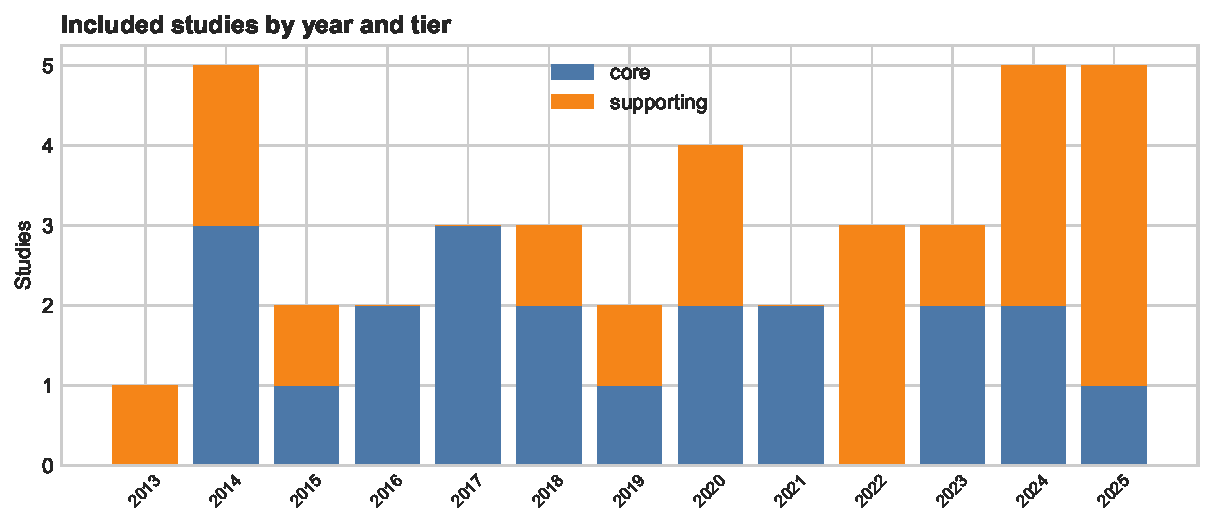
\includegraphics[width=\linewidth]{figures/year_tier.pdf}\end{subfigure}
\begin{subfigure}{0.48\textwidth}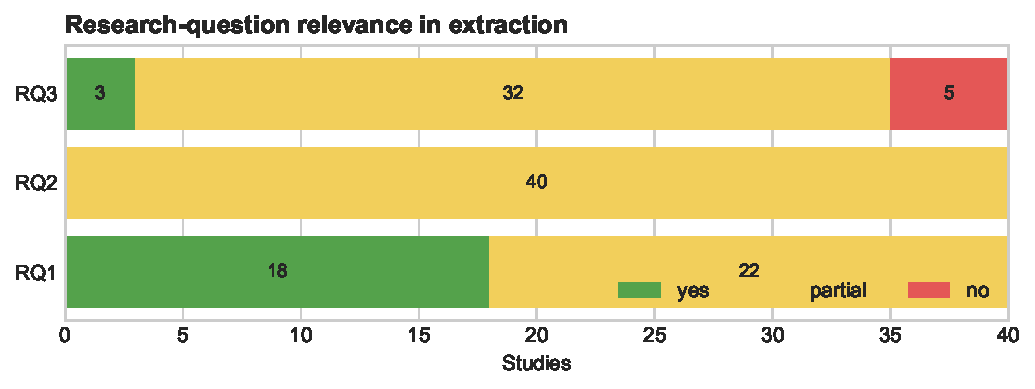
\includegraphics[width=\linewidth]{figures/rq_relevance.pdf}\end{subfigure}
\begin{subfigure}{0.48\textwidth}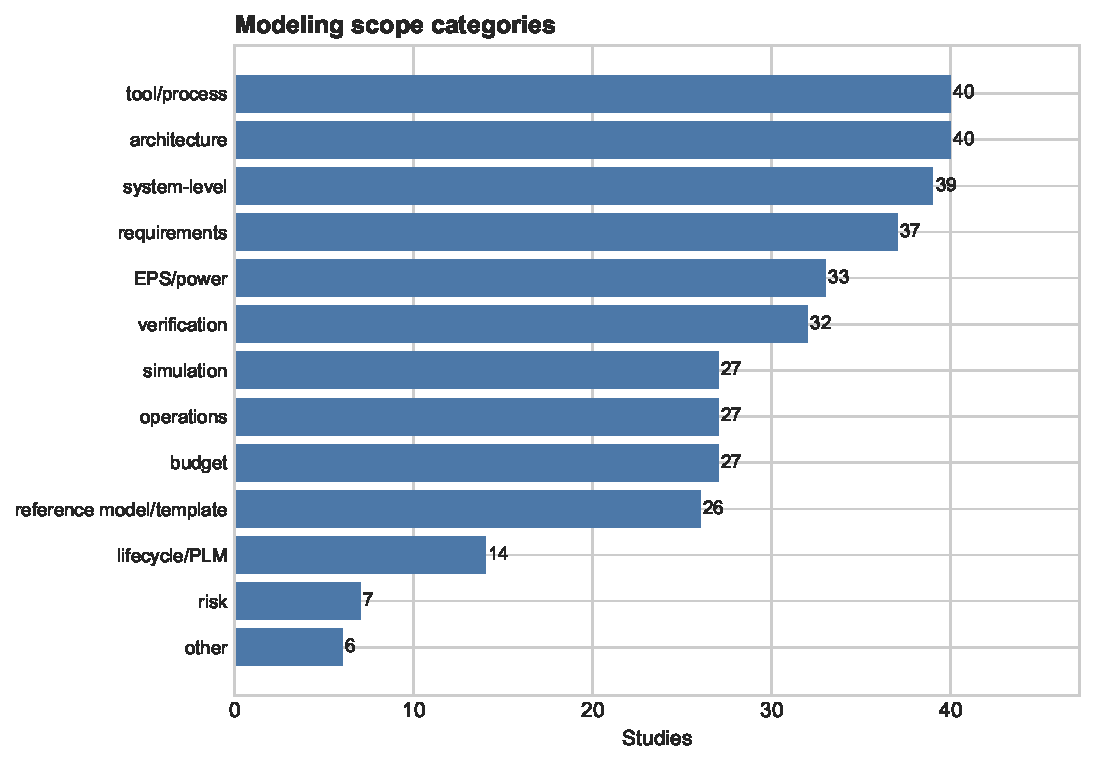
\includegraphics[width=\linewidth]{figures/scope_categories.pdf}\end{subfigure}
\begin{subfigure}{0.48\textwidth}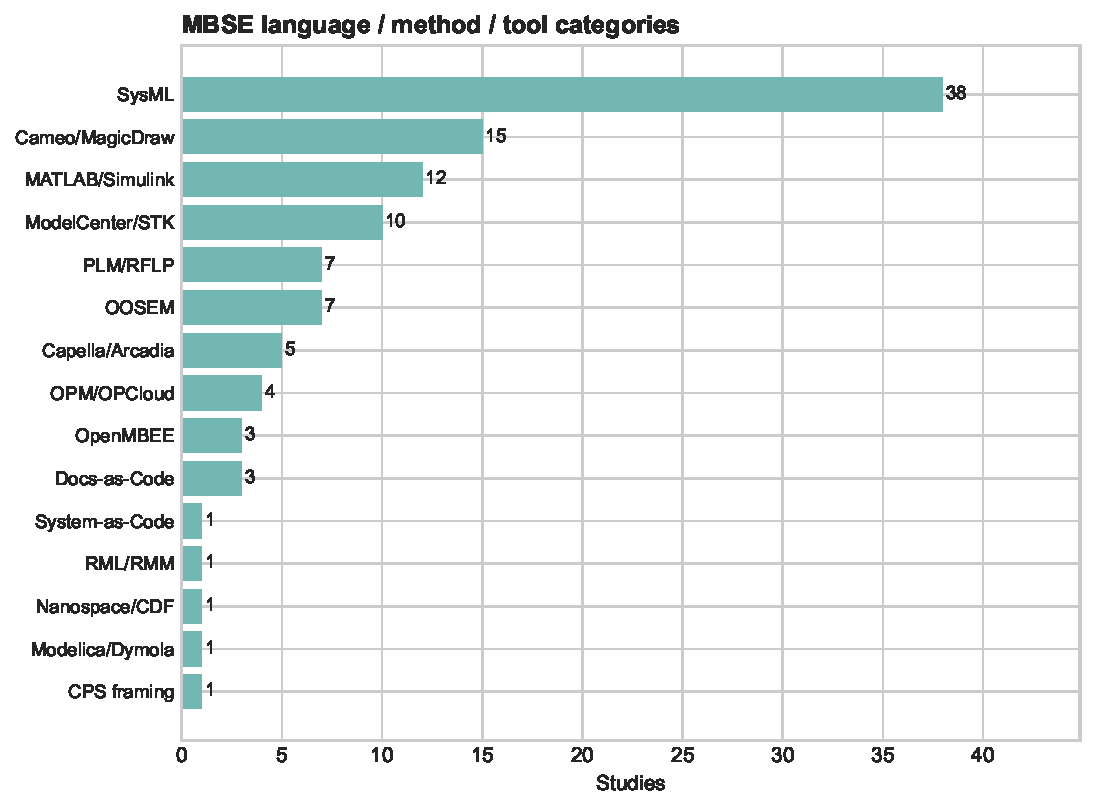
\includegraphics[width=\linewidth]{figures/tool_categories.pdf}\end{subfigure}
\caption{Study years, RQ relevance, modeling scope, and MBSE language/method/tool categories.}
\end{figure}

\begin{figure}[htbp]
\centering
\begin{subfigure}{0.48\textwidth}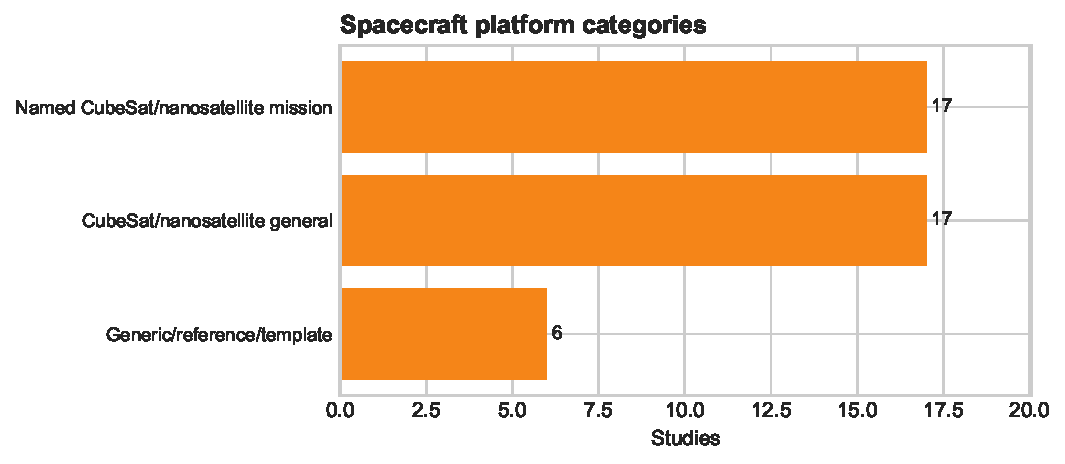
\includegraphics[width=\linewidth]{figures/platform_groups.pdf}\end{subfigure}
\begin{subfigure}{0.48\textwidth}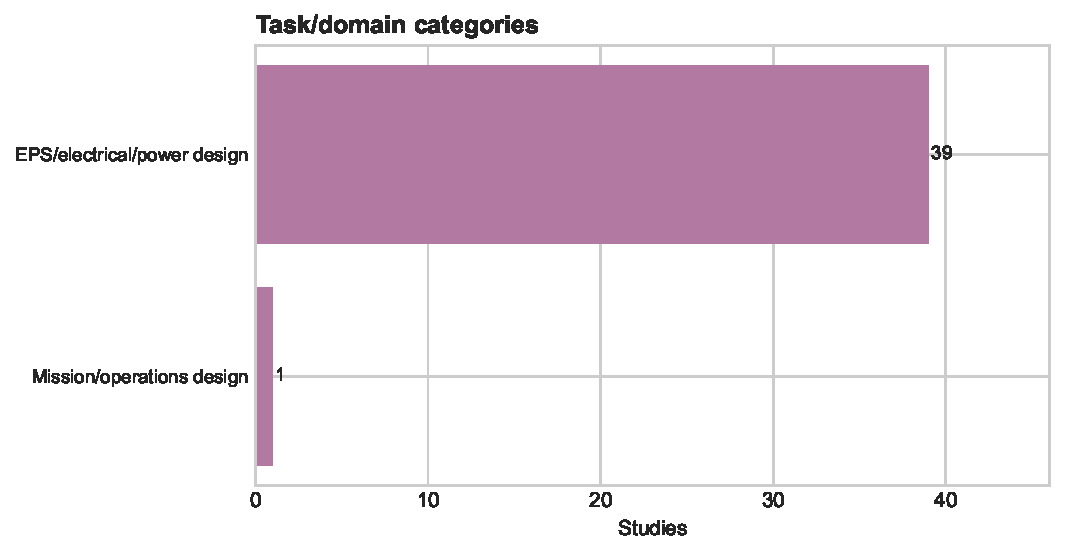
\includegraphics[width=\linewidth]{figures/task_domains.pdf}\end{subfigure}
\begin{subfigure}{0.48\textwidth}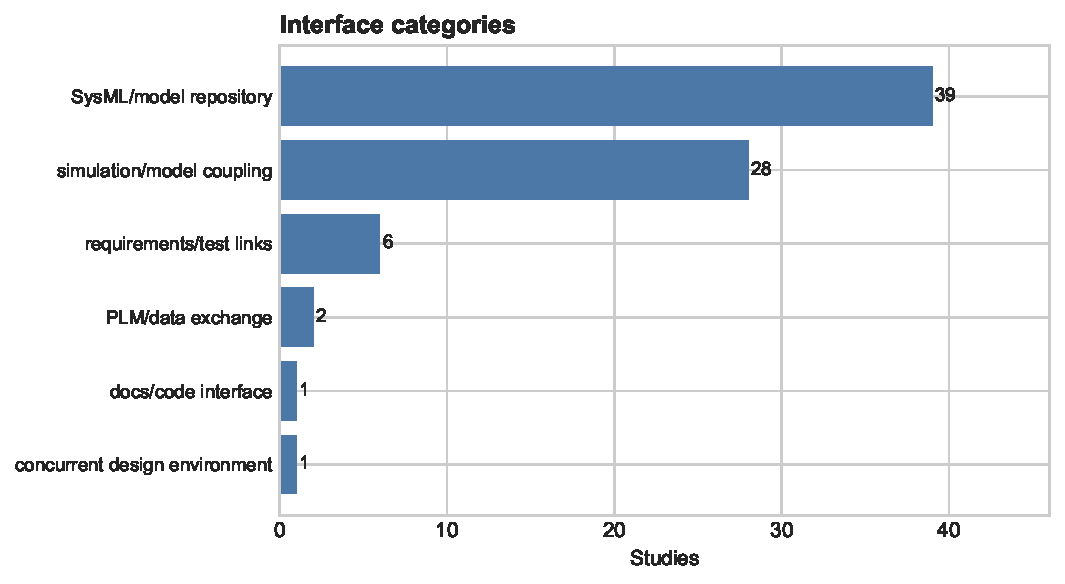
\includegraphics[width=\linewidth]{figures/interface_categories.pdf}\end{subfigure}
\begin{subfigure}{0.48\textwidth}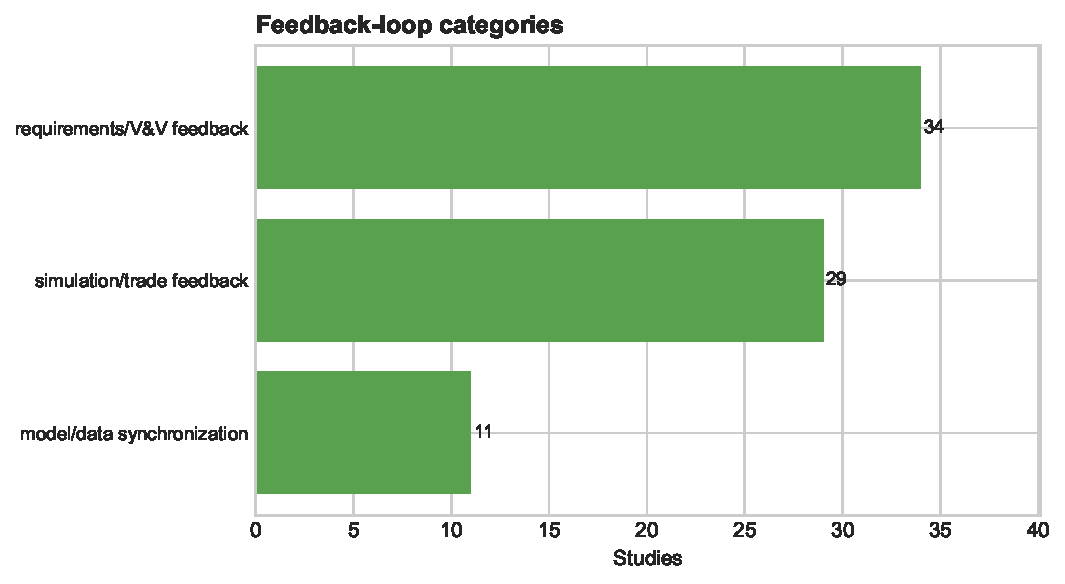
\includegraphics[width=\linewidth]{figures/feedback_categories.pdf}\end{subfigure}
\caption{Platform, task/domain, interface, and feedback-loop categories.}
\end{figure}

\begin{figure}[htbp]
\centering
\begin{subfigure}{0.48\textwidth}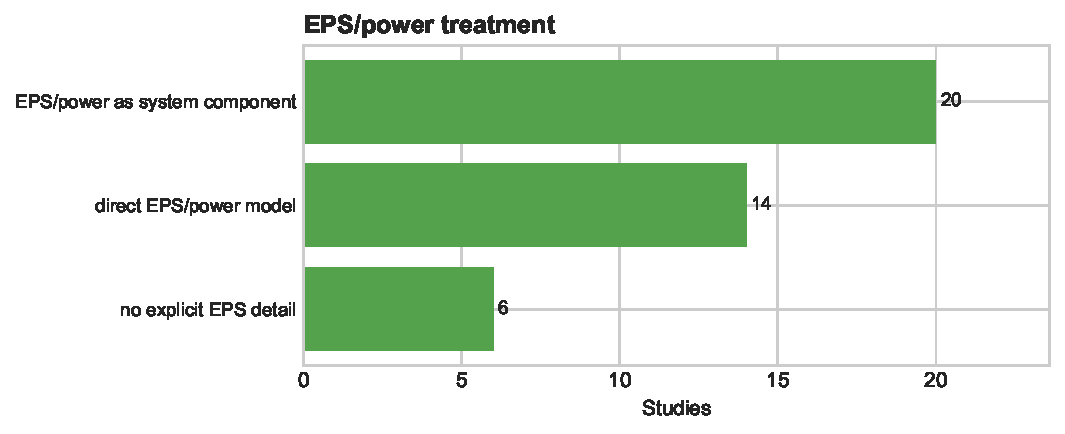
\includegraphics[width=\linewidth]{figures/eps_level.pdf}\end{subfigure}
\begin{subfigure}{0.48\textwidth}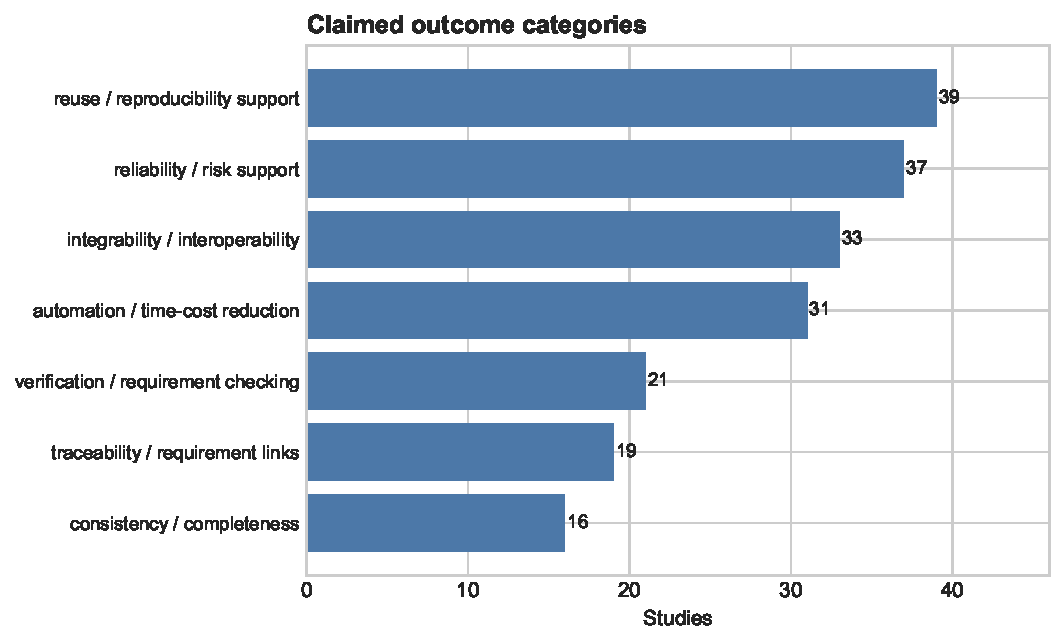
\includegraphics[width=\linewidth]{figures/outcome_categories.pdf}\end{subfigure}
\begin{subfigure}{0.48\textwidth}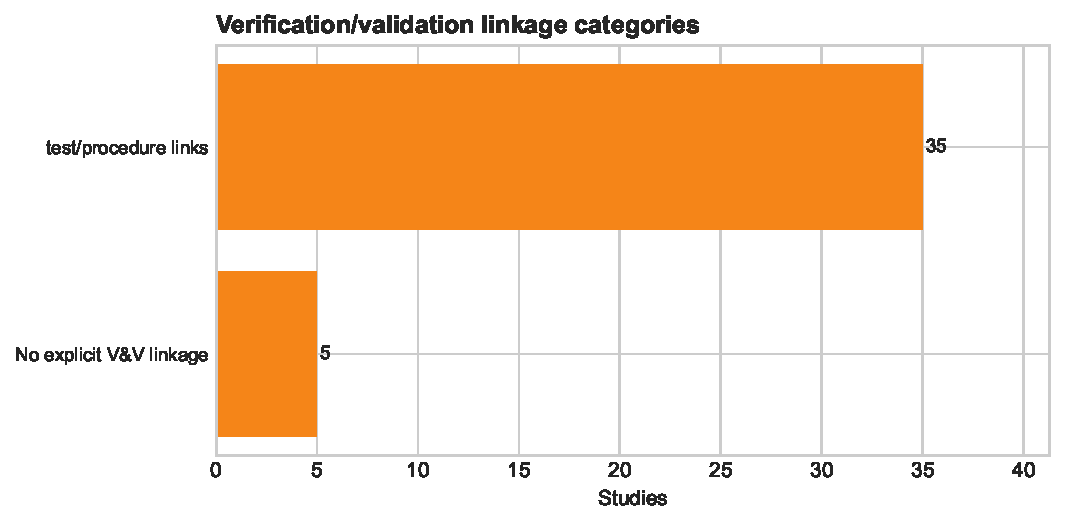
\includegraphics[width=\linewidth]{figures/vv_categories.pdf}\end{subfigure}
\begin{subfigure}{0.48\textwidth}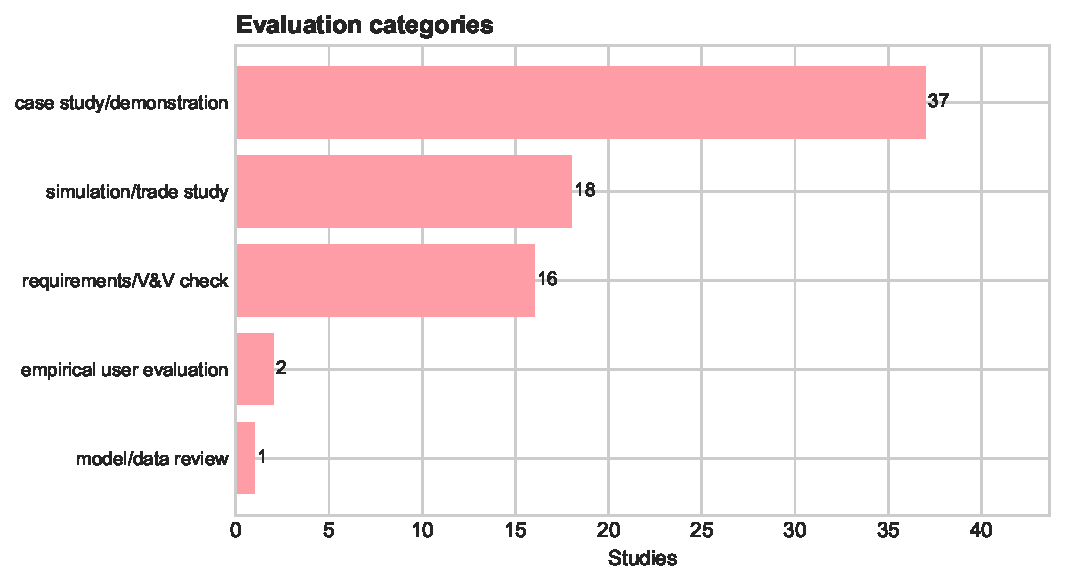
\includegraphics[width=\linewidth]{figures/evaluation_categories.pdf}\end{subfigure}
\caption{EPS treatment, claimed outcomes, V\&V linkage, and evaluation categories.}
\end{figure}

\begin{figure}[htbp]
\centering
\begin{subfigure}{0.48\textwidth}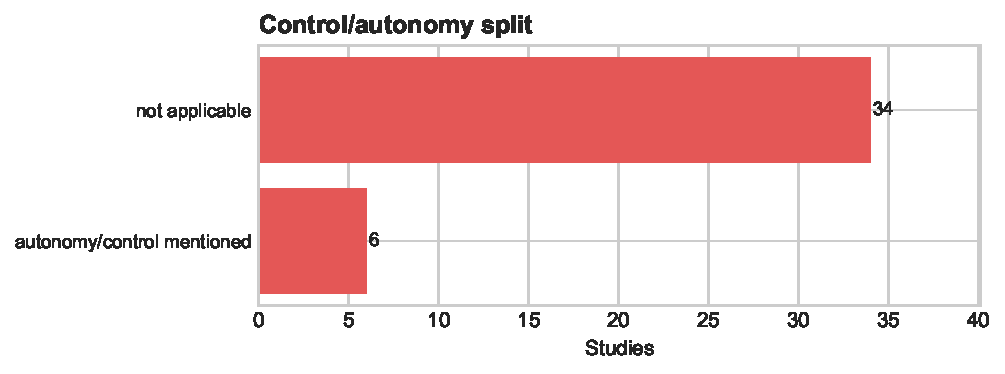
\includegraphics[width=\linewidth]{figures/control_autonomy.pdf}\end{subfigure}
\begin{subfigure}{0.48\textwidth}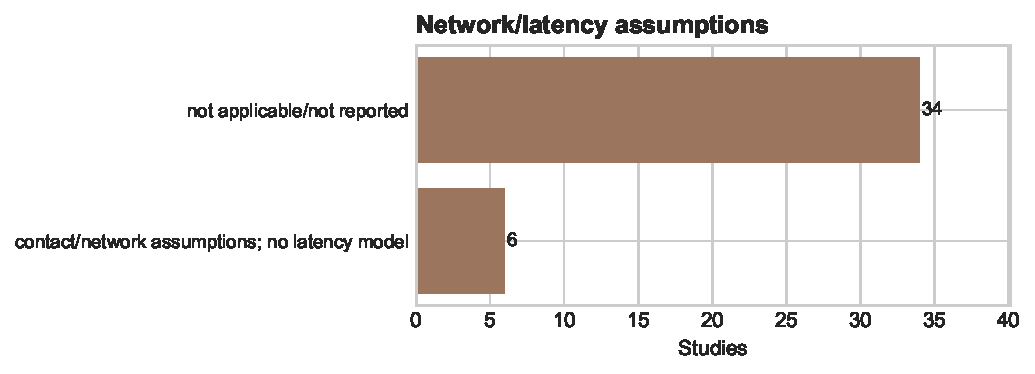
\includegraphics[width=\linewidth]{figures/network_latency.pdf}\end{subfigure}
\begin{subfigure}{0.48\textwidth}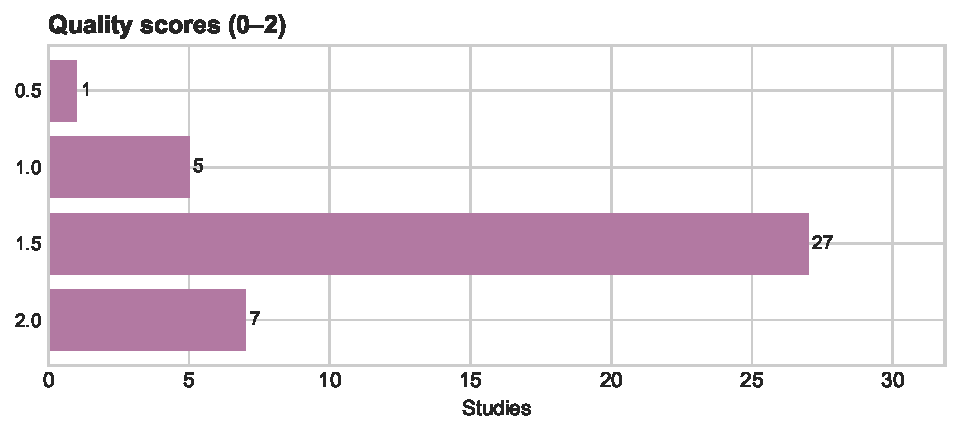
\includegraphics[width=\linewidth]{figures/quality_scores.pdf}\end{subfigure}
\begin{subfigure}{0.48\textwidth}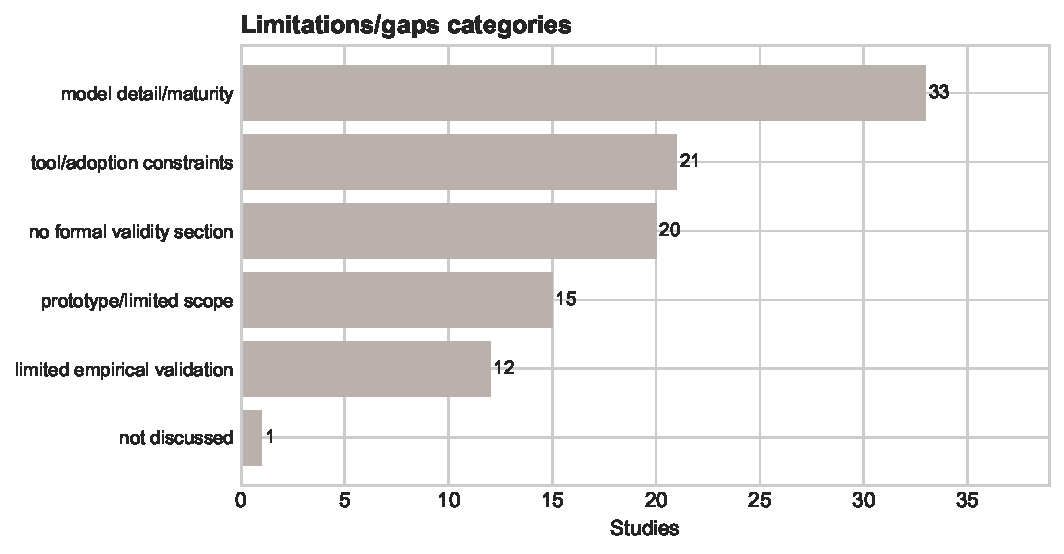
\includegraphics[width=\linewidth]{figures/limitations_categories.pdf}\end{subfigure}
\caption{Control/autonomy, network/latency, quality, and limitation categories.}
\end{figure}

\clearpage
\section*{Included sources}
\small
\begin{longtable}{p{1.7cm}p{4.0cm}p{1.1cm}p{1.6cm}p{4.0cm}p{1.2cm}}
\toprule
Study & Citation & Year & Tier & Type & Quality\\
\midrule
\endfirsthead
\toprule
Study & Citation & Year & Tier & Type & Quality\\
\midrule
\endhead
paper-0001 & Kaslow et al. (2014) & 2014 & core & Conference/proceedings & 1.5 \\
paper-0002 & Kaslow et al. (2017) & 2017 & core & Conference/proceedings & 1.5 \\
paper-0003 & Spangelo et al. (2013) & 2013 & supporting & Conference/proceedings & 2.0 \\
paper-0004 & Kaslow et al. (2015) & 2015 & core & Conference/proceedings & 1.5 \\
paper-0005 & Kaslow et al. (2017) & 2017 & core & Conference/proceedings & 1.5 \\
paper-0007 & Kaslow et al. (2018) & 2018 & supporting & Conference/proceedings & 1.0 \\
paper-0008 & Anderson et al. (2014) & 2014 & core & Conference/proceedings & 1.5 \\
paper-0010 & Edmonson et al. (2014) & 2014 & supporting & Conference/proceedings & 1.5 \\
paper-0011 & Kaslow et al. (2020) & 2020 & core & Conference/proceedings & 1.5 \\
paper-0012 & Lowe and Macdonald (2014) & 2014 & supporting & Journal & 2.0 \\
paper-0013 & Kaslow et al. (2018) & 2018 & core & Conference/proceedings & 1.5 \\
paper-0014 & Kaslow et al. (2021) & 2021 & core & Conference/proceedings & 1.5 \\
paper-0015 & Kaslow and Madni (2017) & 2017 & core & Conference/proceedings & 1.5 \\
paper-0016 & Kaslow et al. (2016) & 2016 & core & Conference/proceedings & 1.5 \\
paper-0022 & Kaslow et al. (2015) & 2015 & supporting & Not reported & 1.0 \\
paper-0023 & Hanafi et al. (2024) & 2024 & core & Journal & 1.5 \\
paper-0024 & Menshenin et al. (2020) & 2020 & supporting & Conference/proceedings & 1.5 \\
paper-0026 & Strobbe et al. (2023) & 2023 & core & Conference/proceedings & 1.5 \\
paper-0027 & Cordero et al. (2022) & 2022 & supporting & Conference/proceedings & 2.0 \\
paper-0029 & Luccisano et al. (2024) & 2024 & core & Journal & 2.0 \\
paper-0031 & Kaslow et al. (2016) & 2016 & core & Conference/proceedings & 1.5 \\
paper-0033 & Almeida et al. (2021) & 2021 & core & Conference/proceedings & 1.5 \\
paper-0034 & Alanazi et al. (2019) & 2019 & supporting & Conference/proceedings & 1.5 \\
paper-0037 & Chiu et al. (2023) & 2023 & supporting & Journal & 1.5 \\
paper-0039 & Gregory et al. (2020) & 2020 & core & Conference/proceedings & 1.5 \\
paper-0041 & Jbara (2025) & 2025 & supporting & Conference/proceedings & 1.5 \\
paper-0043 & Campioli et al. (2025) & 2025 & supporting & Journal & 1.5 \\
paper-0046 & Peters et al. (2022) & 2022 & supporting & Conference/proceedings & 1.5 \\
paper-0053 & Boan (2025) & 2025 & supporting & Not reported & 0.5 \\
paper-0054 & Nardi et al. (2025) & 2025 & supporting & Journal & 1.5 \\
paper-0059 & Rehman and Fortin (2024) & 2024 & supporting & Not reported & 1.0 \\
paper-0061 & Bella et al. (2024) & 2024 & supporting & Conference/proceedings & 1.5 \\
paper-0063 & Akarapu et al. (2023) & 2023 & core & Conference/proceedings & 1.5 \\
paper-0068 & Menshenin et al. (2020) & 2020 & supporting & Conference/proceedings & 1.5 \\
paper-0071 & Nagabhushan et al. (2022) & 2022 & supporting & Conference/proceedings & 1.0 \\
paper-0077 & Kaslow et al. (2019) & 2019 & core & Conference/proceedings & 1.0 \\
paper-0078 & Buitrago-Leiva et al. (2024) & 2024 & supporting & Journal & 2.0 \\
paper-0079 & Guo et al. (2014) & 2014 & core & Conference/proceedings & 1.5 \\
paper-0080 & Waseem and Sadiq (2018) & 2018 & core & Conference/proceedings & 2.0 \\
paper-0081 & Mastropietro et al. (2025) & 2025 & core & Conference/proceedings & 2.0 \\
\bottomrule
\end{longtable}
\normalsize

\section*{Findings by research question}
\begin{center}
\begin{tabular}{p{1.3cm}p{10.2cm}p{3.8cm}}
\toprule
RQ & Evidence pattern & Representative sources\\
\midrule
RQ1 & Reusable reference/template models; executable mission models; open data/model architectures. & \cite{paper-0004,paper-0011,paper-0039,paper-0001,paper-0033,paper-0029,paper-0081} \\
RQ2 & Reported outcomes: traceability, integrability, budget consistency, reuse, requirement-check visibility; measured EPS reliability gains are rare. & \cite{paper-0026,paper-0041,paper-0053,paper-0001,paper-0027,paper-0078,paper-0080} \\
RQ3 & Main integration route: requirements traceability plus simulation/parametric checking; broader V\&V/test links are usually system-level. & \cite{paper-0001,paper-0026,paper-0033,paper-0015,paper-0034,paper-0059} \\
\bottomrule
\end{tabular}
\end{center}

\section*{Cross-study patterns and limitations}
\begin{itemize}
\item Consensus: studies repeatedly model requirements, architecture, interfaces, behaviors/operations, budgets, and verification links as connected model elements.
\item Tooling pattern: no single toolchain dominates; SysML/Cameo is common, with Capella/Arcadia, OPM/OPCloud, PLM/RFLP, Modelica/Dymola, docs-as-code, and system-as-code variants also present.
\item Common evaluations: case-study CubeSat missions, reference models, preliminary-design budgets, power/data simulations, requirement traceability, and model-review demonstrations.
\item Limitations: one core test/evaluation paper and three supporting papers were inaccessible; RQ2 and RQ3 remain limited by the small number of directly EPS-focused studies.
\end{itemize}

\begin{landscape}
\section*{Extraction matrix I: scope, tools, platform, interface, feedback, autonomy, latency}
\scriptsize
\setlength{\tabcolsep}{2pt}
\begin{longtable}{p{1.1cm}p{3.1cm}p{2.5cm}p{3.3cm}p{4.0cm}p{3.5cm}p{2.8cm}p{2.8cm}}
\toprule
Study & Scope categories & Tools/methods & Platform & Interface & Feedback & Control/autonomy & Network/latency\\
\midrule
\endfirsthead
\toprule
Study & Scope categories & Tools/methods & Platform & Interface & Feedback & Control/autonomy & Network/latency\\
\midrule
\endhead
paper-0001 & system-level, EPS/power, requirements, architecture, budget & SysML, Cameo/MagicDraw, MATLAB/Simulink, ModelCenter/STK & Radio Aurora Explorer (RAX), a three-unit CubeSat mission/platform developed by SRI International and the Michigan Exploration Laboratory; the author… & Tool/model integration interface between MagicDraw SysML diagrams, Cameo Simulation Toolkit behavioral execution, MBSE Analyzer, ModelCenter, STK, MATLAB, and Java scripts. Requirements are… & During behavioral simulation, the top-level activity steps through time; UpdateStates calls MBSE Analyzer to execute ModelCenter-backed parametric diagrams; returned state values… & Not applicable & Ground-station network assumptions are modeled for downlink trade studies, including station locations, altitude, minim… \\
paper-0002 & system-level, requirements, architecture, operations, reference model/template & SysML, Cameo/MagicDraw & Generic CubeSat mission/platform, framed as the CubeSat Mission Enterprise/CubeSat Enterprise; paper describes the 1U CubeSat standard and scalabilit… & Actor/model and mission interfaces are modeled: a Chief Scientist actor invokes CubeSat Enterprise use cases; SysML refine relationships connect requirements, use cases, and activities; act… & Recursive refinement/decomposition is described from mission requirements to use cases to activities and down to lower levels of the mission hierarchy. No simulation feedback loop… & Not applicable & Not applicable \\
paper-0003 & system-level, EPS/power, requirements, architecture, budget & SysML, Cameo/MagicDraw, MATLAB/Simulink, ModelCenter/STK & RAX CubeSat/nanosatellite mission, including RAX-1 and RAX-2; paper describes CubeSats as standardized one-to-three-cube nanosatellites but does not… & Tool/model integration interfaces among MagicDraw SysML models, CST, ParaMagic, STK, PHX ModelCenter, MATLAB, Excel/Mathematica; model repository/collaboration interfaces; flight-ground com… & Model execution supports run-view-update loops: solved parametric values can be updated back to SysML, analyses can be automatically rerun with updated parameters, expected behavi… & Ground operations generate command sets/schedules; the onboard computer processes uploaded commands and dispatches them… & Ground station visibility, line-of-sight access, uplink/downlink states, and ground network parameters are modeled; no… \\
paper-0004 & system-level, EPS/power, requirements, architecture, budget & SysML, Cameo/MagicDraw, MATLAB/Simulink, ModelCenter/STK & CubeSat/nanosatellite spacecraft platform; generic CubeSat Reference/Project Model, with prior application to RAX, a three-unit CubeSat, and planned… & SysML model integration with discipline-specific engineering models and COTS modeling/simulation tools; model also identifies space-ground, launch service, communication service, and payloa… & Prior RAX simulations time-stepped scenarios, sent signals, updated state values, and supported trade studies by varying solar panel area, battery capacity, orbital altitude, and… & Not applicable & Not applicable \\
paper-0005 & system-level, EPS/power, requirements, architecture, verification & SysML & CubeSat/nanosatellite platform; CubeSat unit described as 10x10x10 cm and about 1.3 kg, with units joined for larger satellites; no named mission. & SysML model interfaces with other models and COTS simulation tools; CRM can link to regulatory/reference SysML models and accommodate ground-station services plus transport, launch, and dep… & Traceability and V\&V loop through stakeholder needs/objectives, requirements, measures, viewpoints, representative mission population, V\&V scenarios, and executable mission scenar… & Not applicable & Not applicable \\
paper-0007 & system-level, EPS/power, requirements, architecture, budget & SysML & CubeSat/nanosatellite-class platform; examples are taken from a CubeSat Reference Model. The mission enterprise includes a ground system, launch syst… & Model-integration interfaces are trace relationships and parametric bindings among stakeholder concerns, mission objectives, requirements, MOE/MOP/TPM properties, constraints, and architect… & Technical measures are described as tracked and assessed to provide insight, early indications of development issues, prediction of performance-requirement satisfaction, risk moni… & Not applicable & Not applicable \\
paper-0008 & system-level, EPS/power, requirements, architecture, budget & SysML, Cameo/MagicDraw, MATLAB/Simulink, ModelCenter/STK & CubeSat/picosatellite platform; general CubeSat framework with Radio Aurora Explorer (RAX) 3U CubeSat as the main example and SwampSat shown as a mis… & Model/tool integration interfaces among SysML, simulation/analysis tools, and PLM repositories; SLIM connects SysML model elements to Windchill/Teamcenter PLM parts/BOMs for comparison and… & Requirements flow-down and CONOPS traceability support iterative design; simulations vary parameters such as solar panel area, battery capacity, orbital altitude, and ground netwo… & Not applicable; the paper shows mission operations states and ground commands but does not analyze autonomous control a… & Not applicable; communications downlink, SNR, and ground-network trades are discussed, but latency assumptions are not… \\
paper-0010 & system-level, requirements, architecture, verification, simulation & SysML & Pico-/nano-class small satellite systems (PNSats), stated as less than 50 kg; no named mission, CubeSat form factor, or EPS platform is reported. & SysML is proposed as a common design language across organizational disciplines and subsystem interfaces; the framework maps requirements, models, simulations, and formal PVS specifications… & Design refinement/analysis loop across abstraction levels: consistency is checked within each abstraction level and traceability/refinement between levels; the process is intended… & Not applicable & Not applicable \\
paper-0011 & system-level, EPS/power, requirements, architecture, budget & SysML, Cameo/MagicDraw, MATLAB/Simulink, ModelCenter/STK & CubeSat/nanosatellite mission platform, including CubeSat form factor and CubeSat deployment system accommodation; prior project history applied the… & Model/interface coverage includes space and ground components, CubeSat deployer interface requirements, requirement relationships to stakeholders/behaviors/technical measures/V\&V, graphical… & Technical measures are tracked and assessed, with verification activities providing data to the technical measurement process. Future feedback from university teams using the CSRM… & Not applicable & Not applicable \\
paper-0012 & system-level, EPS/power, requirements, architecture, budget & Cameo/MagicDraw, MATLAB/Simulink & CubeSat/nanosatellite mission platform; CubeSat mass range 1-10 kg and discrete 1U, 2U, 3U...NU sizing are discussed. Case studies are an Earth-obser… & Model/data-flow interface through a design structure matrix linking optimizer, inputs/constants, trajectory, space segment, launch segment, ground segment, and performance blocks. User-defi… & The controlled elitist genetic algorithm manipulates mission inputs to improve objective functions, while iterative/numerical loops in Matlab solve directed model relationships. T… & Not applicable & Not applicable; the paper discusses ground-station visibility, communication duty cycle, and data rates, but not commun… \\
paper-0013 & system-level, EPS/power, requirements, architecture, verification & SysML, Cameo/MagicDraw, MATLAB/Simulink, ModelCenter/STK & CubeSat/nanosatellite platform; general CRM for mission-specific CubeSat teams. Paper notes 1U and larger CubeSat form factors such as 3U, 6U, and 12… & Table-based user interfaces in Cameo Systems Modeler for adding, deleting, and modifying mission, specification, requirements, structures, and use-case information; XMI import/export interf… & Technical-measure feedback loop in which verification activities provide data to assess MOEs/MOPs/TPMs, and parametric diagrams can support performance analysis. CRM validation al… & Not applicable & Not applicable \\
paper-0014 & system-level, EPS/power, requirements, architecture, verification & SysML & CubeSat/nanosatellite mission/platform; space and ground segments. No specific CubeSat form factor or named mission is reported. & Model/tool interface: mission teams download the CSRM specification/files from OMG and import them into their own graphical modeling tool. Model integration interfaces include trace links a… & Trade-study/technical-measure feedback is described: performance levels derived from requirements and technical measures are used to make mission-level decisions and measure decis… & Not applicable & Not applicable; downlink data rate and data timeliness are discussed qualitatively, but no latency assumptions are repo… \\
paper-0015 & system-level, EPS/power, requirements, architecture, verification & SysML, OOSEM & CubeSat/nanosatellite platform; CubeSat described as a low-cost standardized nanosatellite, basic 1U unit 10x10x10 cm and about 1.3 kg, with 1U/2U/3U… & Model interfaces include stakeholder viewpoints, requirements traceability, space/ground segment and subsystem relationships, Ground Station Services and Transport/Launch/Deploy Services, s… & Technical measures are modeled as measurable block value properties that can be compared with target values. V\&V workflow uses viewpoints as objective evidence, a CRM populated wi… & Not applicable & Not applicable \\
paper-0016 & system-level, EPS/power, requirements, architecture, budget & SysML, Cameo/MagicDraw, OpenMBEE, OOSEM & CubeSat/nanosatellite reference platform; generic CubeSat unit/form-factor discussion with mission-specific CubeSat models; prior phases applied the… & Reference model feeds mission-specific CubeSat models; SysML model interfaces with COTS modeling and simulation tools; distribution mechanisms include MagicDraw/ZIP/XMI/OpenMBEE/Teamcenter;… & Concept trade-study process identifies parameters driving MOEs, MOPs, and TPMs and then carries out trades; distributed model context includes user feedback mechanisms; SysML mode… & Not applicable & Not applicable \\
paper-0022 & system-level, EPS/power, requirements, architecture, budget & SysML, Cameo/MagicDraw, OpenMBEE, OOSEM & CubeSat/nanosatellite platform; generic CubeSat Reference Model. Paper notes 1U, 2U, and 3U CubeSats as common, newer 6U/12U/27U specifications, and… & System model is described as integrating discipline-specific engineering models and simulations; mission model can interface with a space-system model such as AGI System Tool Kit for input… & Trade-study loop uses model parameters to drive external space-system analysis and return quantifying outputs; state, parametric, and activity diagrams are then used to establish… & Not applicable & Not applicable \\
paper-0023 & system-level, EPS/power, requirements, architecture, budget & SysML, Cameo/MagicDraw, MATLAB/Simulink, ModelCenter/STK & MASAT1 Moroccan university nanosatellite/CubeSat mission, including space segment, ground segment, platform subsystems, payload, and a 1U CubeSat mas… & SysML model interfaces include requirements-to-design and requirements-to-verification trace links, package/diagram organization, and subsystem data, power, and service flows. The EPS inter… & Iterative needs/requirements/ConOps refinement and functional-breakdown loops are modeled. Requirements tables/matrices provide satisfaction and verification feedback. Operational… & The model includes onboard autonomy requirements: automatic space-segment supervision, at least 36 hours of operation w… & Not applicable \\
paper-0024 & system-level, architecture, lifecycle/PLM, tool/process, other & SysML, PLM/RFLP, OPM/OPCloud & Small satellite/CubeSat Earth Observation Mission; form factor and named mission not reported. & Model/data integration interface among OPM conceptual design, CPM PLM representation, and STEP AP 242 detailed design; downstream correspondences are represented through a DSM. STEP AP 242… & Thermal-control example represents sensors, controller, heating/cooling processes, and state changes based on measured temperature thresholds; no simulation or V\&V feedback loop i… & Not applicable & Not applicable \\
paper-0026 & EPS/power, requirements, architecture, budget, verification & SysML & CubeSat/nanosatellite power subsystem; no named mission; form factor not explicitly stated, though CubeSat standards from 1U to 12U and an assumption… & Papyrus model/diagrams and tables; Papyrus .uml file is input to Java code; output is traceability table(s)/Excel with parameter old/new values and requirement-constraint status. & Scenario-based analysis loop: user changes parameter values, code recalculates dependent power-budget parameters and flags constraints as respected/not respected. No closed-loop o… & Not applicable & Not applicable \\
paper-0027 & system-level, EPS/power, requirements, architecture, budget & SysML, Capella/Arcadia, OPM/OPCloud, Nanospace/CDF & CubeSat/nanosatellite platform; CREME CubeSat Radiation Environment Monitoring Experiment in LEO; paper explores 2U feasibility and then 3U design sc… & Nanospace web GUI, database, and API for parameter storage, data sharing, third-party expert software exchange, and envisioned integration with an MBSE tool through API links to budgets, re… & Dependency graph and DSM show feedback loops and indicate which script parts/design parameters must be rerun or updated after unmet requirements; simulations feed intermediate res… & Not applicable & Not applicable \\
paper-0029 & system-level, EPS/power, requirements, architecture, budget & SysML & CubeSat/nanosatellite spacecraft platform; proof-of-concept case is The White Compass (TWC), a theoretical academic concept with a constellation of 1… & Tool/model integration interface: UML stereotypes encode design parameters in the SysML/Gaphor model file; a parser extracts them into a software-readable database used by Nanostar or other… & The parser can be reversed to update model files after analysis or optimization, and generated dependency graphs show how changes in one variable affect other model elements; simu… & Not applicable & Not applicable \\
paper-0031 & system-level, EPS/power, requirements, architecture, verification & SysML, Cameo/MagicDraw, OpenMBEE, OOSEM & CubeSat/nanosatellite platform. The paper defines CubeSats as miniature spacecraft based on a 10-cm unit cube, about one kilogram per cube, typically… & The paper states that MBSE integrates requirements and interfaces in a single system model and helps integrate discipline-specific engineering models and simulations. It also identifies dis… & Model updates are described as automatically propagated into system views; previous phases executed behaviors and constraint equations for operational trade studies. The distribut… & Not applicable & Not applicable \\
paper-0033 & system-level, EPS/power, requirements, architecture, budget & SysML, Capella/Arcadia, CPS framing & General CubeSat-based space missions; demonstrated on NanosatC-Br2 (NCBR2), a 2U CubeSat mission. & Users create and parameterize a Capella Class Diagram Mission Architecture Model; the C2F plugin is invoked from a Capella context menu to generate a Julia script for ForPlan; ForPlan simul… & Iterative model-simulation-analysis loop: define mission elements and equipment operations, create/parameterize the MAM, convert it to a ForPlan script, simulate, analyze battery… & Not applicable; the paper defines equipment operation functions for simulation but does not discuss autonomous operatio… & Ground-station visibility and data transfer rates are modeled for downlink; communications latency assumptions are not… \\
paper-0034 & system-level, requirements, architecture, verification, tool/process & SysML, RML/RMM & CubeSat system; NDSAT example/test satellite concept; background notes CubeSat form factors from 1U to 6U. & RMM maps between process flows, business objectives/rules, requirements, code, and test cases. OBC subsystem connection to communication/data handling and EPS is mentioned, but interface de… & Test cases and defects are mapped back to requirements/business requirements/test scenarios; RMM is described as helping identify requirements with frequent defects and missing li… & Not applicable & Not applicable \\
paper-0037 & system-level, EPS/power, requirements, architecture, verification & SysML, Docs-as-Code & SeaLion 3U CubeSat mission/platform, a joint ODU, USCGA, and AFIT CubeSat with three payloads; original paper content is based on the prior VLEO miss… & YAML model files interface with document-generation tools and version-control workflows; generated diagrams/tables are used for team communication. Operationally, data structures model info… & Model-to-document feedback is described: edits to YAML model files can immediately regenerate diagrams, tables, and documents while keeping dependencies in sync. Operational feedb… & Not applicable & Not applicable \\
paper-0039 & system-level, EPS/power, requirements, architecture, budget & SysML, Cameo/MagicDraw & PSAT1U, a 1U CubeSat-class educational satellite/nanosatellite platform intended as a modular architecture for student-built missions. & Model interfaces include subsystem/component relationships in CAMEO/SysML, documented architecture packages, and payload physical/electrical envelope constraints. EPS-related interfaces inc… & The paper demonstrates model change propagation: editing a component such as the watchdog timer specification propagates through defined relationships to the power subsystem and o… & Not applicable & Not applicable; VHF uplink/downlink link budgets are reported, but no network latency assumptions are discussed. \\
paper-0041 & system-level, EPS/power, requirements, architecture, budget & SysML, OPM/OPCloud & CubeSat nanosatellite platform; paper describes the 1U-12U CubeSat standard and demonstrates with ISISPACE CubeSat subsystem data (Antenna System, TR… & Nanosatellite Builder/user enters component attribute data in OPCloud ahead of time or at run time; values may be simulated; inputs/outputs can use Excel; OPL text provides a natural-langua… & Computed budgets are compared with thresholds; subprocesses return a value or "Error", and Decision Making changes Component Selection between accepted and not-accepted. The abstr… & Not applicable & Not applicable \\
paper-0043 & system-level, EPS/power, requirements, architecture, budget & SysML, Capella/Arcadia & FIRE-EYE CubeSat/small-satellite wildfire-monitoring mission; multi-satellite constellation for the Mediterranean region. The extracted text renders… & Integration interface between Capella/ARCADIA MBSE models and external simulations through PVMT-defined properties and a custom Python parser extracting subsystem/component parameters, func… & Simulation outputs and requirement-verification results are fed back into the architecture and operational model. The paper describes feedback that can revise subsystem duty cycle… & Not applicable; the paper models operating modes, commands, on-board processing, and fault-related transitions, but it… & Not reported; near-real-time service and latency are mentioned as stakeholder/system constraints, but no explicit netwo… \\
paper-0046 & system-level, EPS/power, requirements, architecture, budget & SysML & SpudNik-1 CubeSat project at the University of Prince Edward Island; form factor not reported. & OPAL provides a JavaFX graphical user interface with a high-level system model scene, subsystem SAPPhIRE model scenes, buttons/links to requirements and BOM, subsystem interface arrows, sel… & The SAPPhIRE representation includes feedforward and feedback causal links between inputs, physical effects, states, organs, and parts. OPAL evaluation tasks required users to tra… & Not applicable & Not applicable \\
paper-0053 & system-level, EPS/power, requirements, architecture, budget & SysML, Docs-as-Code & 16U nanosatellite in low-Earth orbit; first system analyses selected an SSO orbit at low altitude between 500 and 600 km. The use case is an agile UV… & Standardized file/model interfaces connect engineers and tools: IDM-CIC and Simu-CIC feed a common database; Simu-CIC outputs CCSDS-like orbital scenario files used by Opalis Flows Manager;… & Iterative simulation and design loop: define subsystem/orbital scenario, allocate power to modes, generate power profile and energy flows, run Opalis energy-balance simulations, t… & Not applicable & Not applicable \\
paper-0054 & system-level, EPS/power, requirements, architecture, budget & SysML & BOREALIS, a 6U CubeSat/nanosatellite mission funded by the Italian Space Agency; 14 kg wet mass considered for transfer studies; LEO operations follo… & Planned Valispace integrated design model is described as an interface for subsystem teams to share real-time updates, requirements, components, budgets, data, and development tracking acro… & Design feedback loop: requirements and constraints define architectural decisions; AD options generate mission concepts; MAU/cost model, tradespace, Monte Carlo, and sensitivity a… & The mission is described as requiring autonomy, but transfer maneuvers would be monitored in real time by the ground se… & No explicit network-latency values or assumptions are reported. The utility model considers communication data rate and… \\
paper-0059 & system-level, EPS/power, requirements, architecture, verification & SysML, PLM/RFLP, Modelica/Dymola & CubeSat case study in Low Earth Orbit; form factor and named mission not reported. & Requirements parameters are defined in ENOVIA and read by CATIA functional/logical engineering, which uses Dymola behavior models; implementation functions transfer information between requ… & A simulation/DOE feedback loop compares model outputs with numerical requirement parameters; if a configuration does not satisfy requirements, another configuration is evaluated.… & Not applicable & Not applicable \\
paper-0061 & system-level, EPS/power, requirements, architecture, budget & SysML, ModelCenter/STK & CubeSat/nanosatellite missions; demonstrated on BOSS, a 12U CubeSat mission to Bennu, plus Geo-Profundo 6U LEO CubeSat and cislunar CubeSat inspector… & Central Data Exchange System links discipline spreadsheets for automated/manual data exchange across mission, system, subsystem, and component levels; all team members can access it, with c… & Iterative design refinement and near-real-time concurrent teamwork are central: subsystem analyses feed the central repository, consistency checks flag shared-input issues, and ea… & BOSS operations mention autonomous attitude and trajectory control and navigation map generation, but no detailed contr… & BOSS is described as communicating with ground stations through the mothership as relay; no network latency assumptions… \\
paper-0063 & system-level, requirements, architecture, verification, simulation & SysML, Cameo/MagicDraw, MATLAB/Simulink, OOSEM & EIRSAT-1, a 2U CubeSat nanosatellite developed by University College Dublin through ESA's Fly Your Satellite! programme. & SysML verification model exchanges data with external test scripts and hardware through interface plugins; the described implementation sends parameters from activity models to a Python cli… & Test outcomes update the requirements compliance matrix/Requirements Table automatically; parametric diagrams validate exchanged data and confirm requirements compliance during te… & Not applicable & Not applicable \\
paper-0068 & system-level, architecture, lifecycle/PLM, tool/process, other & PLM/RFLP, OPM/OPCloud & Generic CubeSat mission/system; Earth-observation CubeSat used as the conceptual example; no form factor reported. & DSM/DMM represents subsystem interfaces, including mechanical and energy interfaces among thermal-control elements; OPM-to-CPM mappings represent information-exchange interfaces between MBS… & The OPM/CPM DSM includes downstream conceptual-to-detailed information flow and upstream detailed-to-conceptual information flow described as feedback. No V\&V feedback loop is rep… & Not applicable & Not applicable \\
paper-0071 & system-level, architecture, budget, verification, risk & SysML & RVSAT-1, described as a student nano-satellite/CubeSat project and as a microbiological payload for ISRO's PSLV Stage-4 orbital platform; form factor… & Model interfaces are mainly SysML navigation/traceability links: subsystem BDDs are hyperlinked with system-level architecture blocks, and risk-management blocks are hyperlinked to risk lay… & Risk-management loop described at process level: risk identification, risk analysis, mitigation-plan formulation, mitigation-plan implementation and risk tracking. The model aggre… & Not applicable & Not applicable \\
paper-0077 & system-level, EPS/power, requirements, architecture, budget & SysML & CubeSat/nanosatellite platform; paper describes CubeSat as 1U with larger 3U, 6U, and 12U form factors, and addresses mission-specific CubeSat space… & Model/tool interface includes CSRM delivery as Foundational CSRM, Web Published CSRM, and CSRM XMI File for mission teams to load into a graphical modeling tool. Engineering interfaces incl… & General assessment loops are described: verification activities provide data for the technical measurement process; CSRM validation is to use RFP requirement satisfaction, SysML m… & Not applicable & Not applicable \\
paper-0078 & system-level, EPS/power, requirements, architecture, budget & SysML, MATLAB/Simulink, ModelCenter/STK, Capella/Arcadia & 3ColStar KiboCUBE Colombia 1U CubeSat/small satellite mission for ISS Kibo deployment; the 1U constraint is approximately 10 x 10 x 10 cm and 1.33 kg… & Capella captures requirements-to-function/component/test-case links and logical/physical interfaces. Technical interfaces include subsystem links such as payload-OBC SPI, OBC-EPS and OBC-AD… & Weekly sprints, sprint reviews, stakeholder feedback, and cross-functional meetings updated the centralized Capella model. The model supports traceability and V\&V feedback through… & ADCS control allocation is discussed as either centralized, with the OBC executing the attitude determination and contr… & Not applicable; communication contacts, data rates, uplink/downlink bands, and link-budget characteristics are discusse… \\
paper-0079 & system-level, EPS/power, requirements, architecture, budget & SysML, MATLAB/Simulink & DelFFi mission within QB50: two identical triple-unit CubeSats/nano-satellites, Delta and Phi, advancing the Delfi-n3Xt platform. & Executable SysML/ParaSolver interface transfers values between Artisan Studio SysML instances and MATLAB/Simulink results; Simulink models are translated to hardware-independent C code and… & Verification and development loops are described: MATLAB results are transferred back to SysML to update requirement status; code verification models feed back into the MBSE envir… & Autonomous formation flying is a mission objective and ADCS/GNC modes are simulated, but no detailed human/autonomy con… & Not applicable \\
paper-0080 & system-level, EPS/power, requirements, architecture, budget & SysML, Cameo/MagicDraw, MATLAB/Simulink, ModelCenter/STK & NSS-1 remote sensing student satellite in the Pakistan National Student Satellite Program; described as a typical nanosatellite-class model, with sys… & Tool/model interfaces include MagicDraw import/export with Microsoft Excel and InterCAX integration that treats MATLAB scripts/functions as SysML constraints and reads results back into the… & Iterative design-analysis loop: parameter values can be imported from spreadsheets into SysML/ParaMagic, solved with a local MATLAB SMT solver for target values such as mass and p… & Not applicable & Not applicable \\
paper-0081 & system-level, EPS/power, requirements, architecture, budget & SysML, Capella/Arcadia, Docs-as-Code, System-as-Code & New Space small-satellite/satellite-platform context; satellite platform selected as System of Interest; pilot with Kongsberg NanoAvionics demonstrat… & Functional and component interfaces/exchanges in Capella; payload-to-standard-platform interface context; Python4Capella/API interface to Capella Java model elements; bidirectional links to… & Iterative validation and refinement of generated model elements and functional libraries; bidirectional data flow allows external data/model updates. No operational closed-loop fe… & Not applicable & Not applicable \\
\bottomrule
\end{longtable}
\normalsize
\end{landscape}

\begin{landscape}
\section*{Extraction matrix II: domain, evaluation, outcomes, V\&V, findings, quality, RQ relevance, limitations}
\tiny
\setlength{\tabcolsep}{2pt}
\begin{longtable}{p{1.0cm}p{2.4cm}p{3.1cm}p{3.7cm}p{3.4cm}p{3.1cm}p{1.0cm}p{1.8cm}p{3.4cm}}
\toprule
Study & Task/domain & Evaluation & Claimed outcomes & V\&V linkage & Key findings & Quality & RQ relevance & Limitations\\
\midrule
\endfirsthead
\toprule
Study & Task/domain & Evaluation & Claimed outcomes & V\&V linkage & Key findings & Quality & RQ relevance & Limitations\\
\midrule
\endhead
paper-0001 & CubeSat space-weather science mission and mission-design trade analysis: RAX studies ionospheric electron-density irreg… & The integrated model is demonstrated by executing representative RAX mission simulations and collecting time histories of system states. Four trade studies vary solar panel area,… & MBSE is claimed to integrate discipline-specific engineering models and simulations and provide a cohesive, consistent source of requirements, design, analysis, and verification.; The integrated SysML/ModelCenter/STK/MA… & SysML requirements are connected to calculated Vehicle value properties with satisfy relationships, including downloadDataMB, energyLowerMargin, maxEnergyCapacity, and maxDataCapacity. Figu… & The paper demonstrates an executable MBSE representation of a CubeSat mission by linking a SysML system model to analytical and high-fidelity simulations through ModelCenter and MBSE Analyz… & 1.5/2 & RQ1 yes; RQ2 partial; RQ3 partial & The authors explicitly state that the RAX modeling is a prototype to prove MBSE applicability and is not intended to be an accurate model of the RAX satellite.; The proof of concept is limi… \\
paper-0002 & CubeSat development and mission behavior definition for collecting, downlinking, post-processing, generating products f… & Demonstrated through worked SysML examples for Collect Mission Data and Distribute Mission Data from the CubeSat Reference Model, including requirements diagrams, use case diagram… & The approach is claimed to provide a repeatable, generalized method for CubeSat development teams using top-down requirements analysis, use-case development, and functional analysis.; The system model is claimed to serv… & General MBSE is defined as supporting requirements, design, analysis, verification, and validation across the life cycle. The actual approach focuses on requirements analysis and functional… & The paper proposes an eight-step MBSE approach for CubeSat behavior definition that begins with mission requirements and ends with a functional architecture modeled as a SysML activity hier… & 1.5/2 & RQ1 yes; RQ2 partial; RQ3 no & Only functional requirements are addressed; nonfunctional and interface requirements are left for future work.; Allocation of behaviors to structural elements is only touched upon and needs… \\
paper-0003 & Space weather mission operations for studying ionospheric plasma field-aligned irregularities using a bi-static radar c… & Demonstrated as a RAX CubeSat case study by executing SysML parametric, state machine, and activity models. Examples include three ParaMagic communication SNR/link scenarios, a PH… & Integrated modeling environment enables automated flow of information between simulators, reducing manual information transfer and supporting rapid evaluation of design configurations and mission scenarios.; Users can e… & General V\&V is explicit: SysML requirements can be traced to design, analysis, and verification elements; the model is said to verify design updates against mission requirements; ParaMagic/… & The RAX SysML model decomposes the CubeSat mission into launch system, environment, mission, flight system, ground system, and operational/logical subsystems, with logical and physical mode… & 2/2 & RQ1 partial; RQ2 partial; RQ3 partial & Appropriate licenses are required for all simulation tools and vendor support was needed.; Creating and testing integration required wrapper files, wrapping models, saving, and reopening mo… \\
paper-0004 & CubeSat mission and system design/development across the lifecycle, including space-ground mission architecture, operat… & Interim status paper demonstrated the reference/project model with SysML diagrams, subsystem tables, and summaries of prior RAX simulations and trade studies. The current referenc… & Integrability: MBSE is claimed to help integrate discipline-specific engineering models and simulations, and past phases showed SysML can interface with special-purpose M\&S tools.; Consistency/traceability: the system m… & The paper links the reference model to SysML elements for requirements, design, analysis, verification, and validation. Cal Poly CubeSat Design Specification items for testing and verificat… & The paper reports the fourth phase of the INCOSE SSWG CubeSat Challenge, aiming to build a generic CubeSat Reference Model and a CubeSat Project Model for mission-specific reuse.; The model… & 1.5/2 & RQ1 yes; RQ2 partial; RQ3 partial & The Phase 2 RAX model lacked the ability to time-step through a behavioral model and determine whether requirements were satisfied throughout the entire RAX mission.; Assessment of MBSE met… \\
paper-0005 & CubeSat mission analysis, design, development, deployment, and operation; includes space/ground segment architecture an… & Interim status paper demonstrates the CRM through SysML package, block, requirements, use case, activity, and V\&V diagrams. Completed empirical evaluation is not reported; future/… & System-level MBSE is claimed to keep requirements and design in the model rather than in independent artifacts, supporting traceability and integration.; CRM logical elements are claimed to be reusable as a starting poi… & The CRM package organization includes validation and verification packages. The paper defines validation and verification, lists verification methods as inspection, analysis, demonstration,… & The CubeSat Reference Model is a SysML logical architecture intended as a reusable starting point for university or other CubeSat teams developing mission-specific logical and physical arch… & 1.5/2 & RQ1 yes; RQ2 partial; RQ3 partial & The CRM is still under development; the current architecture has been developed down to subsystems and includes a segment-level mission data collection/distribution use case, while model el… \\
paper-0007 & CubeSat systems engineering and technical measurement for assessing mission objectives such as operational lifetime/ser… & The paper evaluates/demonstrates the approach through worked SysML examples from the CubeSat Reference Model, including mission enterprise MOEs for service life and total cost, Cu… & MBSE/model-centric approach is claimed to provide enhanced communications, reduced development risk, improved quality, and enhanced knowledge transfer.; The technical-measures approach is claimed to provide clear tracea… & General system-level linkage only. The paper states that MBSE supports verification and validation, that MOEs are used to validate user needs, MOPs verify requirements, and TPMs assess prog… & The paper presents a SysML technical-measures profile for stakeholder concerns, mission objectives, MOE/MOP/TPM specifications, and mop/tpm value-property stereotypes.; The proposed flow de… & 1.0/2 & RQ1 partial; RQ2 partial; RQ3 partial & The abstract states that little literature ties technical measurement and MBSE together and that existing literature treats the topic generally and without details.; The related-work sectio… \\
paper-0008 & CubeSat mission/system design, enterprise modeling, conceptual design trades, cost estimation, ground and flight archit… & The paper demonstrates the framework through the RAX CubeSat lineage and described use cases: prior behavioral simulations for communication, power, and mission states; integrated… & MBSE/SysML is claimed to support stronger, more integrated communication between engineering teams.; A CubeSat modeling framework is claimed to allow more robust and reusable designs and to serve as a starting point for… & General MBSE is defined as supporting verification and validation. The integrated analysis architecture is said to enable requirements verification for mission scenarios; reported requireme… & The paper extends an INCOSE Space Systems Working Group CubeSat MBSE framework toward enterprise concerns such as cost, schedule, requirements, stakeholders, ground systems, and lifecycle m… & 1.5/2 & RQ1 yes; RQ2 partial; RQ3 partial & The earlier behavioral-modeling phase lacked the ability to time-step through a behavioral scenario to determine requirement satisfaction across the entire scenario.; CubeSat cost estimatio… \\
paper-0010 & High-confidence design methodology for small satellite space-mission systems, described as cyber-physical sensing platf… & Conceptual/methodological demonstration. The paper defines the RFD framework and verification formulation, then illustrates PVS specification, refinement, and a type-correctness p… & High-confidence/correct-by-construction small-satellite designs through integration of formal methods and MBSE.; Responsiveness to system requirement/specification changes through an agile model-based design process.; I… & General system-level V\&V is central to the proposed process. SysML is proposed for design analysis, simulation, and V\&V; PVS is used from mission objective to mission concept phases; consis… & The paper frames pico-/nano-class small satellites as cyber-physical systems whose resource constraints and subsystem interactions require integrated model-based design.; The RFD process li… & 1.5/2 & RQ1 partial; RQ2 partial; RQ3 partial & The paper explicitly states that formal methods cannot fix incorrect assumptions made in the design phase.; The paper explicitly states that formal methods are not a panacea and that costs… \\
paper-0011 & CubeSat mission architecture and system engineering for space and ground components, targeted especially at university… & The paper demonstrates the CSRM through a notional top-down application outline, diagrams of packages/architecture/V\&V, prior application to RAX and trade-study history, formal re… & Quality enhancements and economies associated with reusability are claimed for adopting the CSRM.; The reusable model is claimed to reduce development times and increase the quality of CubeSat spacecraft and ground-syst… & The CSRM includes a Validation Verification package. Requirement elements expose a Verified By property, and requirements can be traced down to validation and verification activities. Verif… & The CSRM is a platform-independent, SysML-compliant MBSE reference model intended as a reusable starting point for CubeSat space and ground logical architecture.; The model structures CubeS… & 1.5/2 & RQ1 yes; RQ2 partial; RQ3 partial & The CSRM provides a library of model elements but does not dictate which elements or relationships to use; the development team must populate the model with maturing elements.; If the five… \\
paper-0012 & Conceptual and early CubeSat mission design, multidisciplinary trade-space search, and multi-objective optimization for… & Two CubeSat case studies demonstrate the architecture: Case I trades ground sample distance against revisit time over altitude for an EO payload and is described as verifying the… & Rapid trade-space exploration through analytical models rather than computationally expensive numerical orbit propagation, with Case II completing 51,000 model iterations in 10 minutes.; Potentially increased mission ro… & Only informal/system-level linkage is reported: the first case study is said to verify the model architecture and show usefulness for trade studies. No formal verification/validation/test/I… & CubeSat modularity and limited capability reduce the number of design variables, making rapid mission-level trade-space search more feasible than for large spacecraft.; A baseline design st… & 2/2 & RQ1 yes; RQ2 partial; RQ3 no & The authors state that the model architecture cannot be completely generalized because each space mission is unique; only a baseline structure can be maintained and modified per use case.;… \\
paper-0013 & CubeSat systems engineering and reference-model development for mission-specific space/ground mission design; prior RAX… & Paper demonstrates the CRM by describing the Cameo implementation, packages, tables, stereotypes, and diagrams. It does not report a completed empirical evaluation; it presents a… & CRM is intended as a reusable starting point for mission-specific CubeSat teams and as a repository for systems engineering artifacts.; Requirements and design are kept in the model rather than independent artifacts, su… & System-level linkage only. Requirement tables expose verify method and verified-by properties, and the paper states that proof of satisfy assertions is accomplished by verify relationships.… & The CRM is a SysML, methodology-agnostic reference/template intended for CubeSat teams to import and specialize into mission-specific models.; The current maturation expands requirements an… & 1.5/2 & RQ1 partial; RQ2 partial; RQ3 partial & The paper states that validating the CRM is difficult without concrete mission-specific models developed using the CRM.; CRM validation is still in progress: trusted partners had seen the c… \\
paper-0014 & CubeSat mission engineering and mission-specific space-ground system design, including logical architecture, physical a… & The paper presents a preliminary qualitative assessment mapping CSRM support to Mission Engineering activities and identifies areas needing further research. It also states that t… & The MBSE/SysML CSRM is intended to foster completeness and economies of scale associated with reusability.; Use of the CSRM is claimed to establish a mechanism to share and reuse components with other design activities.… & General system-level V\&V linkage is present. The CSRM traces requirements from stakeholders to behaviors, assigns technical measures to subsystems/components for validation and verification… & CSRM is a SysML-compliant MBSE reference model providing a logical CubeSat space-ground architecture without imposing physical implementation constraints.; The CSRM is not pre-populated wit… & 1.5/2 & RQ1 yes; RQ2 partial; RQ3 partial & The paper states that extending CSRM beyond descriptive mission modeling to dynamic analytical assessment of overall mission performance would be challenging and requires much further resea… \\
paper-0015 & Generic CubeSat mission analysis, design, development, deployment, and operations across space and ground segments; mis… & The paper demonstrates the CRM concept through SysML-style views/figures of the CubeSat domain, space and ground segments, requirements hierarchy, mission-specific development flo… & The CRM is intended to facilitate CubeSat design, verification, and validation.; The CRM is intended to support customization for specific CubeSat missions by mission-specific teams.; Providing a standard Reference Mode… & Strong general V\&V linkage. The CRM contains validation and verification packages; mission-specific teams develop a validation and verification approach; validation and verification are def… & The CubeSat Reference Model is a generic MBSE/SysML reference model for the CubeSat mission domain, intended as a starting point for mission-specific CubeSat teams.; The CRM models CubeSat… & 1.5/2 & RQ1 partial; RQ2 partial; RQ3 partial & Further research is needed into how to augment the CRM with other models for CubeSat test and evaluation.; The paper states challenges including no agreed-upon process for developing a Cube… \\
paper-0016 & CubeSat space mission systems engineering, reference architecture development, and concept life-cycle mission design/tr… & Interim/status demonstration through described SysML reference-model artifacts and prior RAX applications: behavior simulations, COTS simulation-tool interfaces, downlink/power tr… & Integrability: the system model helps integrate discipline-specific engineering models and simulations, and prior phases interfaced with COTS simulation tools.; Consistency/configuration: requirements and design are con… & General system-level V\&V linkage only. MBSE is defined as supporting verification and validation; the model includes a Tester stakeholder responsible for V\&V, Cal Poly testing requirements… & The paper presents an interim status of an INCOSE SSWG CubeSat MBSE Reference Model intended as a generic SysML/OOSEM logical architecture for future CubeSat developers.; The current model… & 1.5/2 & RQ1 yes; RQ2 partial; RQ3 partial & The paper states that the fourth-phase modeling effort starts anew.; The effort to date has focused on nomenclature, stakeholder content, measures, and generic architecture down to logical… \\
paper-0022 & CubeSat concept-lifecycle mission and system design, including stakeholder/MOE analysis, logical architecture, mission… & Primarily descriptive/reference-model development paper. It demonstrates intended application through a concept-lifecycle trade-study workflow and cites prior RAX-phase trade stud… & MBSE system model is claimed to be a single source for architecture development and interface management.; The system model is claimed to integrate discipline-specific engineering models and simulations.; The reference… & General linkage only. The paper defines MBSE as supporting verification and validation from conceptual design onward, shows validation as part of reference-model development, and depicts mi… & The paper positions a CubeSat Reference Model as a SysML/OOSEM logical architecture that CubeSat teams can tailor into mission-specific models.; The model scope includes stakeholders, needs… & 1.0/2 & RQ1 partial; RQ2 partial; RQ3 partial & The paper states that a fully formed CubeSat Reference Model could be overwhelming for mission-specific teams, especially teams new to MBSE and SysML.; The reference model had not yet been… \\
paper-0023 & Academic nanosatellite mission preparation, project management, mission analysis, requirements engineering, product/wor… & Qualitative demonstration through application to the MASAT1 mission analysis and PBS modeling case. The paper illustrates SysML package, requirements, BDD, IBD, state-machine, and… & MBSE and SysML are claimed to improve mission reliability by focusing on engineering aspects of projects.; MBSE is claimed to provide better traceability, design consistency, quality improvement, and reduced document ma… & The framework includes lifecycle reviews (MCR, MRR, SDR, PDR, CDR, SAR, PRR, ORR, DR), a Verification package, and requirements tables with Satisfied By and Verified By columns. The Verifie… & The paper adapts ECSS/NASA-style project breakdown and lifecycle practices into a simplified MBSE framework for student-driven academic nanosatellite projects.; The framework organizes nano… & 1.5/2 & RQ1 yes; RQ2 partial; RQ3 yes & Not discussed as a formal limitations or threats-to-validity section.; Explicit future work states that viability and practicality of the PBS model should be improved by integrating externa… \\
paper-0024 & Conceptual-to-detailed design digital-engineering integration for a CubeSat Earth-observation mission; MBSE/PLM data-fl… & Analytical demonstration: extracts 23 entities from OPM, CPM, and STEP, maps full/partial correspondences with DSM, summarizes frequency of entity appearance, and illustrates the… & MBSE/PLM integration is claimed to facilitate better data flow from conceptual design to detailed design.; A well-integrated MBSE/PLM chain is claimed to help store design heritage and track how system architecture chan… & No paper-specific verification, validation, IVV, or test procedure linkage is demonstrated. The paper states in background that SysML diagrams support verification and validation, but its a… & OPM represents conceptual system information with objects, processes, states, and relationships; the paper treats states as linking object/space and process/time representations.; CPM and S… & 1.5/2 & RQ1 partial; RQ2 partial; RQ3 no & The authors explicitly scope the analysis to unidirectional data flow from conceptual design to detailed design and include only downstream correspondences.; The authors call the analysis a… \\
paper-0026 & Early/conceptual CubeSat electrical power subsystem design, power budget analysis, requirements traceability, and model… & Demonstration on a Papyrus SysML CubeSat power subsystem model. The authors apply the Java code to a power-budget scenario with assumptions and user updates (solar panel length an… & Model-based traceability lets designers see how parameter changes affect other parameters and whether requirements are met.; The open-source Papyrus implementation is claimed to make the modeling effort more accessible… & EPS-specific model-based requirement verification is integrated through SysML requirements/constraints, assumptions, constraint blocks, and a Java code that extracts data from the Papyrus .… & The paper presents a Papyrus SysML model of a CubeSat power subsystem organized into requirements, structure, behavior, and analysis packages.; The modeled EPS architecture includes electri… & 1.5/2 & RQ1 partial; RQ2 partial; RQ3 yes & Only nominal behavior is shown; mission modes are explicitly not discussed, although the authors say the methodology could be extended to them.; Activity diagrams and state machine diagrams… \\
paper-0027 & Concurrent preliminary design of CubeSats, using the CREME radiation-monitoring CubeSat as a case study; mission/orbit,… & Demonstrated through the CREME simplified but real CubeSat use case, SysML/DSM experiment, and semi-automated Python/GMAT/Dosa/Stela/Celestlab analyses. Iterations check power DoD… & MBSE may let Nanospace reuse knowledge, accelerate design convergence, and speed inspection of candidate architectures.; Claimed MBSE benefits include better communication/information sharing, increased traceability and… & General MBSE definition and discussion link modeling to requirements, design, analysis, verification, and validation. In the CREME case, simulations check requirements/constraints before ph… & The paper frames Nanospace as an open-source web CDE environment for academic CubeSat preliminary design and examines early MBSE integration challenges.; CubeSat preliminary design is repre… & 2/2 & RQ1 partial; RQ2 partial; RQ3 partial & Only a subset of CREME requirements and constraints is considered because of space constraints.; Mission modes are not discussed, although the authors state the concept could be extended to… \\
paper-0029 & Concurrent preliminary design of CubeSat missions; case-study mission domain is GNSS service provision across the Arcti… & Demonstrated through an end-to-end proof-of-concept on the TWC theoretical mission: the SysML model is parsed into a database and linked to NSS tools to generate power and data bu… & A generic CubeSat SysML model with UML stereotypes can serve as a central data source or single source of truth throughout preliminary design.; The parser enables integration between the CubeSat model and open-source si… & No explicit EPS-specific verification, test, or IVV procedure model is provided. The paper defines MBSE as supporting verification and validation, includes SysML requirements and a parser-g… & The proposed framework has three main steps: characterize data in a CubeSat SysML model through UML stereotypes, parse the model file into a software-readable data structure, and use the da… & 2/2 & RQ1 yes; RQ2 partial; RQ3 partial & The parser is tailored to Gaphor model files and cannot automatically extract data from models developed with other tools without source-code modification.; The operating-mode generalizatio… \\
paper-0031 & Generic CubeSat mission and systems engineering reference model for future CubeSat developers, educational use, and eva… & Status/progress paper rather than quantitative validation. It demonstrates the approach through summarized prior phases: SysML application to RAX, behavior simulation, interfaces… & Integrability: the system model is claimed to integrate discipline-specific engineering models and simulations and to keep requirements and interfaces in a single model.; Change consistency: the paper claims that change… & General V\&V linkage is present. The paper defines MBSE as supporting requirements, design, analysis, verification, and validation across the lifecycle; the stakeholder model includes a Test… & The INCOSE SSWG Challenge Team is developing a CubeSat Reference Model as a SysML logical framework for future CubeSat developers.; The reference model scope includes mission stakeholders,… & 1.5/2 & RQ1 yes; RQ2 partial; RQ3 partial & The paper states that the earlier FireSat example was hypothetical, so a real space system could not be built from that model and practical use could not be demonstrated or verified.; The C… \\
paper-0033 & Phase-0/Pre-Phase A mission concept and ConOps analysis; operational scenario simulation; power and data budget balanci… & Demonstrated through the NanosatC-Br2 2U CubeSat case. The authors generated and iterated a MAM, transformed it with C2F, ran ForPlan simulations, and inspected battery charge and… & Operations simulations generated from the MAM can be used in Phase-0 mission concept analyses to verify initial operations requirements and drive later design implementation.; C2F integrates Capella MAMs with ForPlan by… & The paper links the model to verification through ForPlan ConOps simulation and an explicit requirements-met iteration. It states that simulations support verification of initial operations… & Academic CubeSat development often skips or rushes systems-engineering practices, including mission concept analyses, which motivates the proposed MBSE/simulation workflow.; The proposed MA… & 1.5/2 & RQ1 yes; RQ2 partial; RQ3 partial & To use the workflow with other satellite simulators, the MAM must be changed to fit the new simulator inputs and C2F must be changed to match the new simulator configuration method.; The cu… \\
paper-0034 & CubeSat requirements analysis, OBC software architecture, radio message handling, and camera image storage test-case ma… & Illustrative case study for a typical CubeSat/NDSAT example using process-flow diagrams, an RMM table for radio and camera functions, OBC functional/nonfunctional requirements, an… & RML is claimed to enhance requirements quality and ease analysis and elicitation.; RML is claimed to help CubeSat developers group and prioritize requirements and identify ambiguity or inconsistency.; RMM is claimed to… & Explicit general V\&V linkage: the RMM maps process steps, requirements, business rules/objectives, code, test-case IDs, tests, and results; the case study is presented as requirements valid… & The paper positions RML as a stakeholder-oriented visual requirements modeling language for CubeSat development rather than a detailed system behavior language.; The RMM traceability struct… & 1.5/2 & RQ1 partial; RQ2 partial; RQ3 partial & Future work will verify and characterize the efficacy of the proposed approach.; Future work will test the approach in an actual project and update it based on that experience. \\
paper-0037 & CubeSat mission and flight-software architecture for on-orbit validation of an Impedance Probe, multispectral sensor, a… & Demonstrated through the SeaLion mission architecture implementation: examples of YAML references, stakeholder needs, user stories, data structures, generated UML diagrams, genera… & The approach is intended to assist improving CubeSat success rates for university teams by making systems engineering tools readily available and usable.; MBSE is claimed to reduce ambiguity from informal language and m… & General system V\&V linkage is present. The paper states that MBSE models were used for design, specification, analysis, verification, and validation. Stakeholder needs and user stories incl… & SeaLion used MBSE with a docs-as-code approach in which YAML model files are the source for generated documents, diagrams, tables, and references.; M30ML was selected because it was lightwe… & 1.5/2 & RQ1 partial; RQ2 partial; RQ3 partial & The published implementation was based on the prior VLEO mission profile and had not yet been updated for the later launch/profile change.; Component implementation was still a work in prog… \\
paper-0039 & CubeSat-class satellite system design and education; reusable/template mission-specific CubeSat development with EPS/po… & The model is demonstrated through PSAT1U examples and screenshots/diagrams: architecture hierarchy, ADCS block definition diagram, EPS package diagram with power budget, watchdog-… & The standardized MBSE template is claimed to make the CubeSat design cycle more efficient and reduce future design/development times.; Defined relationships are claimed to propagate system changes automatically and avoi… & General linkage only. The introduction quotes the standard MBSE definition including support for requirements, design, analysis, verification, and validation across lifecycle phases, and cl… & The paper develops a PSAT1U baseline MBSE model from the CSRM as a standardized template for CubeSat-class satellites.; The baseline model defines important PSAT1U subsystems, components, a… & 1.5/2 & RQ1 yes; RQ2 partial; RQ3 partial & No formal limitations or threats-to-validity section is provided.; The paper explicitly notes that teaching students all of MBSE and tool use is beyond the scope of the course. \\
paper-0041 & Conceptual CubeSat design support: budget calculation for mass, volume, height, and power; component-selection complian… & The model is demonstrated in OPCloud by executing an OPM model with real ISISPACE subsystem specifications. Animated execution traces budget calculations, a valid case sets Compon… & Automation and significant shortening of the CubeSat budget-calculation/component-screening process.; Formal model makes the budget-calculation process clear, unambiguous, and understandable through graphical OPM and OP… & General model/tool V\&V linkage only. OPCloud is said to provide visual simulation engines supporting validation, verification, and testing. The paper verifies/demonstrates the budget model… & The proposed OPM model represents Budget Calculating at the top level with CubeSat NanoSatellite System, Nanosatellite Builder, Component Selection states, and output budget objects.; Budge… & 1.5/2 & RQ1 partial; RQ2 partial; RQ3 partial & The paper states that the work is not comprehensive and uses selected budget calculations to demonstrate the automated budget-calculation tool.; The paper describes the model as a proof of… \\
paper-0043 & Preliminary design, analysis, and simulation-driven validation of a wildfire detection and monitoring space mission, in… & Case-study demonstration on the FIRE-EYE wildfire-monitoring mission. The authors build Capella OA/SA/LA/PA models and use extracted model data for orbital coverage/access, power… & Improved traceability, reusability, and simulation fidelity across the system lifecycle are stated as framework goals.; Improved consistency between system models and simulation artifacts, reduced integration costs, and… & General V\&V: simulation is embedded for design-space exploration, performance and functional verification, operational consistency checks, and low-level requirement verification; simulation… & MOSAiC integrates ARCADIA/Capella MBSE with open-source, multi-domain simulation environments for space-system design and analysis.; The framework uses Actor, System, Subsystem, and Compone… & 1.5/2 & RQ1 partial; RQ2 partial; RQ3 partial & No formal limitations or threats-to-validity section is provided; limitations are mostly implicit in challenges and future-work statements.; The work is presented as a first version of MOSA… \\
paper-0046 & CubeSat conceptual design support, concurrent conceptual design data management, subsystem behavior modeling, causal tr… & The authors surveyed SpudNik-1 conceptual design files, built OPAL as a proof-of-concept, and tested it with 15 UPEI engineering students. Participants received about a 15-minute… & Integrability/data integration: OPAL was designed as a central data repository incorporating files from all six SpudNik-1 subsystems and integrating code, analysis, spreadsheet, CAD, and other file types.; Traceability… & No spacecraft or EPS verification/test/IVV procedure is integrated into the model. The study evaluates the OPAL tool through student usability/task testing. The paper explicitly states that… & The SpudNik-1 conceptual design file survey found EPS-related data that could be mapped to SAPPhIRE elements, including requirements, power budget spreadsheets, solar-panel data sheets, and… & 1.5/2 & RQ1 partial; RQ2 partial; RQ3 no & The file survey found no appropriate file corresponding to the Physical Phenomena element, likely because subsystem experts did not explicitly share qualitative behavior descriptions.; The… \\
paper-0053 & Preliminary electrical architecture and EPS sizing for an agile nanosatellite science mission requiring repeated observ… & The workflow is demonstrated on a specific 16U nanosatellite use case. CNES flight-dynamics experts reduce the annual observation plan to a representative 48-hour worst-case sun-i… & The process defines an adaptable and interoperable model, allowing mission changes to be studied almost instantly by regenerating ephemeris data and configuration changes to be compared easily.; A common database lets s… & The linkage is simulation-based rather than formal V\&V. The EPS model, power profile, and ephemeris-derived energy flows are used to validate energy feasibility of observation plans, demons… & The paper frames electrical architecture work as part of a concurrent engineering process in which a common technical reference for satellite description and mission supports system-level b… & 0.5/2 & RQ1 partial; RQ2 partial; RQ3 partial & Not discussed \\
paper-0054 & Astrobiology/space biology CubeSat mission design: in-orbit lab-on-chip study of microbial biofilms under microgravity… & Demonstrated as a BOREALIS case study. Preliminary GMAT mission analysis, FLUKA/SPENVIS/IRENE radiation/dose analysis, and COTS-derived subsystem data feed a MAU/cost model over 1… & MBSE/tradespace approach is claimed to support robust, data-driven decisions that optimize mission architecture for performance and cost.; The structured workflow is claimed to ensure traceability and repeatability and… & General system-level linkage only. The paper lists development and verification plans as SE outputs for validation against mission requirements and operational readiness checks; it also ben… & BOREALIS is a 6U CubeSat mission with a lab-on-chip and fluorescence microscope payload for microbial biofilm experiments in LEO and MEO.; The MBSE model represents the system through archi… & 1.5/2 & RQ1 partial; RQ2 partial; RQ3 partial & The model contains subjective weight assignments based on engineering judgment, although the authors test robustness with Monte Carlo and sensitivity analysis.; The authors warn that if the… \\
paper-0059 & Conceptual/early-phase CubeSat product development and requirements traceability, focused on electrical power behavior,… & Design research methodology prescriptive study demonstrated through a CubeSat case in 3DExperience. The authors create a simulation scenario after deployment/detumbling, feed ecli… & Requirements-in-loop and requirements traceability across requirements, functional, logical, and physical RFLP stages in a PLM tool.; Timely decision support through DOE-generated configurations and simulation-based che… & General V\&V is linked through numerical requirement parameters, digital tests, behavior simulation, and DOE. EPS-specific verification is explicit: SoC must remain above 60\%, Dymola/simulat… & The paper demonstrates an RFLP implementation in 3DExperience for a CubeSat, linking requirements in ENOVIA to functional/logical SysML architecture, Dymola behavior models, and physical ar… & 1.0/2 & RQ1 partial; RQ2 partial; RQ3 yes & The case study is limited to a single CubeSat viewpoint focused on the electrical power view.; The launch segment was not considered because the study concentrated on the spacecraft part. \\
paper-0061 & Preliminary phase 0/A CubeSat mission and system design for space exploration and observation, including BOSS asteroid… & The approach was implemented and tested in several CubeSat case studies, with BOSS described in detail through four concurrent design sessions. Effectiveness is assessed by compar… & Faster, more flexible, and transparent design management compared with traditional methods, simplifying system design flow and early decision-making.; Early model integration is claimed to allow system compatibility ass… & General linkage only: CE/MBSE tools are said to improve design, development, and verification, and early model integration is said to let verification begin in advance. The paper does not d… & The proposed methodology combines concurrent engineering with MBSE to support phase 0/A CubeSat design through simultaneous system modelling and iterative refinement.; The S3D Tool provides… & 1.5/2 & RQ1 yes; RQ2 partial; RQ3 partial & The paper states that the S3D Tool needs improvement and optimisation.; The Optical Payload calculation sheet needs updating and integration into the central repository, and dedicated sprea… \\
paper-0063 & CubeSat lifecycle MBSE and Phase C-D satellite-ground communications subsystem requirements verification/testing. & Preliminary demonstration on the EIRSAT-1 communications subsystem. The paper describes using a SysML verification model based on a traditional end-to-end test plan, integrating i… & A single integrated MBSE environment is claimed to ensure verification is planned and executed in the correct sequence with full requirements traceability.; System models are claimed to integrate with external programma… & The paper explicitly links MBSE with verification and validation. The EIRSAT-1 model includes a Verification and Validation package; the demonstrated MBSE verification model is based on a t… & The NSM project seeks MBSE coverage across the CubeSat lifecycle from Phase A/B conceptualization through Phase C/D testing and verification to Phase E launch and operations.; The EIRSAT-1… & 1.5/2 & RQ1 partial; RQ2 partial; RQ3 partial & The paper states that few standards exist for systems engineering in nanosatellite design and development, apart from limited case studies and academic articles.; The paper states that no s… \\
paper-0068 & Space mission architecture and digital engineering information exchange from conceptual design to detailed design; Cube… & Case-study demonstration on a CubeSat: OPM/OPCloud conceptual CubeSat decomposition, DSM/DMM thermal-control subsystem interface/state/process representation, CPM radiator detaile… & Reduced complexity and errors and improved efficiency are claimed as capabilities of digital transformation/information exchange, but not quantitatively evaluated.; Integration of MBSE approaches and PLM methods through… & Not reported/none. The paper demonstrates a case-study information-exchange model but does not link the model to verification, validation, IVV, testing, or EPS verification procedures. & A DSM-based approach is proposed to manage digital engineering information exchange for CubeSat space-mission architecture.; OPM/OPCloud is used for conceptual CubeSat and subsystem modelin… & 1.5/2 & RQ1 partial; RQ2 partial; RQ3 no & No formal limitations or threats-to-validity discussion is reported.; The paper frames application to more complex systems, a concurrent engineering design environment, and extended lifecyc… \\
paper-0071 & Risk management and systems engineering for a student nanosatellite/CubeSat mission, including technical, schedule, fun… & Demonstrated as a proposed SysML framework/template for RVSAT-1 in Eclipse Papyrus with figures for the model tree, system context diagram, subsystem attributes layer, risk identi… & The proposed risk model is claimed to enable ease of access and optimization so systems engineers can focus on value-added risk-management tasks.; The layered and hyperlinked SysML structure is claimed to provide seamle… & General system-level V\&V linkage only. The paper quotes the INCOSE MBSE definition including support for verification and validation, states SysML supports verification and validation, and… & RVSAT-1 previously used a document-based tailored Risk Response Matrix with risk description, severity, likelihood, response strategy, trigger and contingency plan.; The proposed method tra… & 1/2 & RQ1 partial; RQ2 partial; RQ3 partial & No explicit limitations or threats to validity of the proposed model are discussed.; Future scope is to interface the model with external tools such as MATLAB Systems Composer and Simulink… \\
paper-0077 & CubeSat mission and system design/development, including space segment, ground segment, mission-specific logical and ph… & The paper demonstrates the CSRM through SysML package/diagram excerpts and defines validation approaches for the CSRM/MSM: OMG RFP requirement satisfaction, Practical Guide to Sys… & CSRM logical components are intended to be reused as a starting point for mission-specific CubeSat logical and physical architecture development.; Using the CSRM for a mission-specific CubeSat is claimed to establish a… & General MSM V\&V is explicitly modeled. Verification Activity elements verify requirements through verify/verifies/verified-by relationships and may capture verification plans, procedures, e… & The CSRM is an INCOSE SSWG CubeSat system reference model and proposed OMG normative specification using SysML for a space-and-ground CubeSat system.; The CSRM provides a reusable logical a… & 1.0/2 & RQ1 yes; RQ2 partial; RQ3 partial & The CSRM is not pre-populated with specific stakeholders, technical measures, use cases, or requirements; mission-specific teams must populate and tailor these elements.; The paper states t… \\
paper-0078 & Preliminary design of a CubeSat mission for space weather/solar wind particle monitoring, IoT connectivity demonstratio… & Case-study demonstration on the 3ColStar preliminary design completed over 4 months. Evaluation/demonstration includes Capella operational/logical/physical architecture diagrams,… & MBSE rigorously managed technical consistency across architectural documents, ensuring coherency and minimizing errors.; Arcadia/Capella digitalized the system as models containing requirements, architecture, and interf… & General system V\&V is explicitly linked to MBSE: requirements are connected to functions, logical components, physical designs, and verification test cases in Capella; V\&V is supported with… & The paper applies Arcadia/Capella MBSE and Agile/Scrum practices to the preliminary design of the 3ColStar 1U CubeSat mission.; The system model includes operational entities, stakeholder n… & 2/2 & RQ1 partial; RQ2 partial; RQ3 partial & Actual manufacturing of the subsystems had not yet started; the work reports preliminary design activities.; The thermal analysis is explicitly described as preliminary and requiring furthe… \\
paper-0079 & Nano-satellite mission and system definition; autonomous formation flying and thermosphere science; ADCS/AOCS/GNC desig… & Demonstrated through the DelFFi case study with SysML mission/system/subsystem requirements, an executable SysML ADCS4simulation parametric model linked to MATLAB/Simulink, and a… & Improved requirements traceability and overall model consistency through SysML requirements tables and diagrams; not EPS-specific.; Reusable model/template approach for nanosatellite development; the paper states templa… & General and ADCS-specific linkage is strong: SysML requirements are refined by constraint blocks and executable parametric diagrams; ParaSolver links Artisan Studio SysML instance values to… & The paper proposes MBSE as a gap-filling methodology for nano-satellite development, using DelFFi as the case study.; SysML stereotypes and requirement diagrams are used to derive customer… & 1.5/2 & RQ1 yes; RQ2 partial; RQ3 partial & Requirement diagrams can become cluttered; the paper recommends partitioning requirements analysis across dedicated diagrams.; The paper reports ambiguity in choosing SysML relations such a… \\
paper-0080 & Conceptual design and systems engineering of a remote sensing student/nanosatellite mission, including requirements, ar… & Demonstrated through an NSS-1 case-study SysML repository and example diagrams. The main worked evaluation is a ParaMagic/MATLAB SMT mass and power budget analysis that computes p… & MBSE is claimed to provide more formal, complete, semantically rich system specifications and design for analysis, verification, and validation from early project phases.; SysML modeling is claimed to improve requiremen… & SysML requirement diagrams define requirements, traceability, and test cases that verify requirements. Mass and power requirements are linked with verify relationships to Mass\_MoS and Power… & The NSS-1 repository uses SysML to represent common nanosatellite design patterns, including values, scenarios, functions, parts, subsystems, and relationships among them.; The model organi… & 2/2 & RQ1 yes; RQ2 partial; RQ3 partial & The paper explicitly states that aerospace system engineers are often less familiar with software engineering, object-oriented programming, SysML, and MBSE tools.; The paper identifies the… \\
paper-0081 & Standardized satellite platform development and payload integration for Satellite-as-a-Service/New Space missions; serv… & Pilot implementation with Kongsberg NanoAvionics on a demonstration mission. The approach was evaluated across satellite platform modeling, functional library development, digital… & Automated framework supports fast, consistent deployment of satellite digital models across missions.; Object-oriented functional analysis plus System-as-Code is claimed to streamline standard satellite-platform develop… & General model/workflow V\&V only. Validation used manual inspection of generated Capella models, Capella built-in model validation tools, and incremental checks of functional libraries and i… & The paper proposes an object-oriented functional modeling approach for New Space satellite platforms, using functional groups derived from use cases as reusable building blocks.; The satell… & 2/2 & RQ1 partial; RQ2 partial; RQ3 partial & Initial modeling effort is higher during transition to a System-as-Code framework.; The custom automation layer is spread across multiple custom APIs and Python classes, creating maintainab… \\
\bottomrule
\end{longtable}
\normalsize
\setlength{\tabcolsep}{6pt}
\end{landscape}

\section*{Column coverage}
\begin{center}
\small
\begin{tabular}{p{5.2cm}p{9.2cm}}
\toprule
Extraction form column & Where presented in this report\\
\midrule
corpus\_id, tier, citation, year, venue/type & Included-sources table; year/tier and venue/type charts\\
Robot platform / spacecraft platform & Platform chart; extraction matrix I\\
Task/domain & Task/domain chart; extraction matrix II\\
Interface & Interface chart; extraction matrix I\\
Feedback & Feedback chart; extraction matrix I\\
Control/autonomy split & Control/autonomy chart; extraction matrix I\\
Network/latency assumptions & Network/latency chart; extraction matrix I\\
Evaluation & Evaluation chart; extraction matrix II\\
Key findings & Extraction matrix II\\
Quality & Quality chart; included-sources table; extraction matrix II\\
RQ relevance & RQ relevance chart; RQ evidence table; extraction matrix II\\
Limitations & Limitations chart; extraction matrix II\\
Protocol-specific fields: modeling scope, MBSE language/method/tool, claimed outcomes, V\&V linkage & Scope, tool, outcome, EPS-treatment, and V\&V charts; extraction matrices I--II\\
\bottomrule
\end{tabular}
\end{center}

\section*{Extraction quality and confidence}
\begin{itemize}
\item Paper-level extraction outputs were valid for 40/40 accessible studies.
\item All required fields were present for every study; RQ relevance values used controlled labels; quality-score totals matched the two checklist subscores.
\item Confidence is highest for RQ1, moderate for RQ2, and moderate-low for RQ3 because direct EPS-specific IVV/test-procedure integration is sparse.
\end{itemize}

\nocite{*}
\printbibliography[title={Sources}]
\end{document}
